% !TEX TS-program = pdflatexmk
\documentclass[12pt]{amsart}

%auto-ignore
%this ensures the arxiv doesn't try to start TeXing here.
%!TEX root=exceptional.tex
\usepackage{amssymb}
\usepackage{array}
\usepackage{booktabs}
\usepackage{mdwtab}
\usepackage{mathtools}
\usepackage[T1]{fontenc}
\usepackage[utf8]{inputenc}
\usepackage{libertine}
\usepackage[libertine]{newtxmath}
\usepackage{hyphenat}
\usepackage{enumitem}
\usepackage{xcolor}
\definecolor{medium-blue}{rgb}{0,0,0.65}
\usepackage{ifpdf}
\ifpdf
  \usepackage[pdftex]{graphicx}
  \usepackage[pdftex,margin=1.25in]{geometry}
  \usepackage[bookmarks=true, bookmarksopen=true,%
    bookmarksdepth=3,bookmarksopenlevel=2,%
    colorlinks=true,%
    linkcolor=purple,%
    citecolor=medium-blue,%
    filecolor=blue,%
    menucolor=blue,%
    urlcolor=medium-blue]{hyperref}
  \hypersetup{pdftitle={Towards the quantum exceptional series}}
  \hypersetup{pdfauthor={Scott Morrison, Noah Snyder, and Dylan P. Thurston}}
\else
  \usepackage[dvips]{graphicx}
  \usepackage[dvips,margin=1in]{geometry}
  % Use hyperref with all features turned off even in DVI mode, since
  % the .aux file format changes
  \usepackage[draft]{hyperref}
\fi
\usepackage{url}
\usepackage{todonotes}
\usepackage{tikz}
\usetikzlibrary{shapes}
\usetikzlibrary{calc}
\usetikzlibrary{knots}

\usepackage[backend=biber,style=alphabetic,doi=false,isbn=false,url=false,minnames=6,maxnames=6]{biblatex}
\setcounter{biburlnumpenalty}{9000}
\setcounter{biburllcpenalty}{1000}
\setcounter{biburlucpenalty}{8000}
\renewbibmacro{in:}{%
  \ifentrytype{article}{}{\printtext{\bibstring{in}\intitlepunct}}}
\renewbibmacro*{volume+number+eid}{%
  \printtext{vol.}
  \printfield{volume}%
  \setunit*{\addnbspace}% NEW (optional); there's also \addnbthinspace
  \printfield{number}%
  \setunit{\addcomma\space}%
  \printfield{eid}}
\DeclareFieldFormat[article]{number}{\mkbibparens{#1}}
\usepackage{silence}
% Filter warnings issued by package biblatex starting with "Patching footnotes failed"
\WarningFilter{biblatex}{Patching footnotes failed}
\addbibresource{bibliography/bibliography.bib}

% A binary operator with a subscript on both sides (and correct spacing)
% Name stands for subscript-operator-subscript
\newcommand{\sos}[3]{\mathbin{{}_{#1}\mathord#2_{#3}}}

% manyindices
% Adapted from code by "bza" in comp.text.tex, Feb. 7, 2006
%% USAGE:
%%
%% \manyindices#1#2#3#4#5
%%
%% #1=lower left index
%% #2=upper left index
%% #3=lower right index
%% #4=upper right index
%% #5=main symbol
\makeatletter
\newcommand\mi@kern[1]{%
  \settowidth\@tempdima{$\mi@obj^{#1}$}
  \kern-\@tempdima
  #1
  \settowidth\@tempdima{$\mi@obj$}
  \kern\@tempdima
}

\newtoks\mi@toksp
\newtoks\mi@toksb
\DeclareRobustCommand{\manyindices}[5]{
  \def\mi@obj{#5}
  \mi@toksp\expandafter{\mi@kern{#2}}
  \mi@toksb\expandafter{\mi@kern{#1}}
  \@mathmeasure4\textstyle{#5_{#1}^{#2}}
  \@mathmeasure6\textstyle{#5_{#3}^{#4}}
  \dimen0-\wd6 \advance\dimen0\wd4
  \@mathmeasure8\textstyle{\hphantom{{}_{#1}^{#2}}#5^{\the\mi@toksp#4}_{\the\mi@toksb#3}}
  \hbox to \dimen0{}{\kern-\dimen0\box8}
}
\makeatother 

% Left sub/super scripts
% \lsup is a temporary definition until something better is worked out
% Use \lsupv if the next argument is vertical
\newcommand{\lsub}[2]{{}_{#1}#2}
\newcommand{\lsup}[2]{{}^{#1}\mskip-.6\thinmuskip#2}
\newcommand{\lsupv}[2]{{}^{#1}#2}
\newcommand{\lsubsup}[3]{\manyindices{#1}{\mskip.6\thinmuskip#2\mskip-.6\thinmuskip}{}{}{\mathord{#3}}}
\newcommand{\lsubsupv}[3]{\manyindices{#1}{\mskip.2\thinmuskip#2\mskip-.2\thinmuskip}{}{}{\mathord{#3}}}

\newcounter{saveenum}

% Read the file, if it exists
\newread\testin
\def\maybeinput#1{
\openin\testin=#1
\ifeof\testin\typeout{Warning: input #1 not found}\else\input#1\fi
\closein\testin
}

\def\mathcenter#1{%
  \vcenter{\hbox{$#1$}}%
}

\def\graph#1{
        \includegraphics{#1}
}

\def\mathgraph#1{
        \mathcenter{\graph{#1}}
}

\def\mfig#1{
        \mathcenter{\includegraphics{#1}}
}

\def\mfigb#1{
        \mathcenter{\includegraphics[trim=-1 -1 -1 -1]{#1}}
}


%%% Local Variables: 
%%% mode: latex
%%% TeX-master: "main"
%%% End: 

\usepackage{fp}
\usepackage{tikz}
\usetikzlibrary{matrix}
\usetikzlibrary{arrows,backgrounds,patterns,scopes,external,hobby,
    decorations.pathreplacing,
    decorations.pathmorphing
}

\newlength{\fuzzwidth}
\setlength{\fuzzwidth}{2.5pt}
\newlength{\arrowlength}
\setlength{\arrowlength}{8pt}
\newlength{\arrowwidth}
\setlength{\arrowwidth}{.75pt}
\newlength{\pointrad}
\setlength{\pointrad}{1.5pt}
\newlength{\linewid}
\setlength{\linewid}{1.5pt}
\newlength{\circlerad}
\setlength{\circlerad}{16pt}
\newlength{\smcirclerad}
\setlength{\smcirclerad}{8pt}
\newcommand{\fillcolor}{black!60}
\newcommand{\fuzzcolor}{black!25}
\newcommand{\arrowcolor}{black!25}
\newcommand{\covercolor}{black!0}
\newcommand{\graycolor}{black!55}
\newcommand{\graylightcolor}{black!40}


\newcommand{\coverwidthfuzz}{6pt}
\newcommand{\coverwidth}{3.5pt}
\newcommand{\coverwidththin}{3.25pt}
\newcommand{\coverwidththick}{3.75pt}

\newlength{\linewidthin}
\setlength{\linewidthin}{1.25pt}
\newlength{\linewidthick}
\setlength{\linewidthick}{1.75pt}


\tikzset{use Hobby shortcut}
\tikzset{
	coverline/.style={
	preaction={draw,line width=\coverwidth,\covercolor}}, 
	coverlinethin/.style={
	preaction={draw,line width=\coverwidththin,\covercolor}}, 
	coverlinethick/.style={
	preaction={draw,line width=\coverwidththick,\covercolor}}, 
	coverlineleft/.style={
	preaction={draw,line width=\coverwidthfuzz,\covercolor,decorate,decoration={curveto,amplitude=0,raise=.35*\fuzzwidth}}}, %%% Notice this number was tweaked, 	
coverlinelefttail/.style={
	preaction={draw,line width=\coverwidthfuzz,\covercolor,decorate,decoration={curveto,amplitude=0,raise=.35*\fuzzwidth,pre=moveto,pre length=2pt}}}, %%% Notice this number was tweaked, probably will not look good if parameters change.  Again here, pre removes the raise option.
        fuzzlefttail/.style={
        preaction={draw,line width=\fuzzwidth,\fuzzcolor,decorate,decoration={curveto,pre=moveto,pre length=2pt,amplitude=0,raise=.5*\fuzzwidth}}}, %%% This does not work --- somehow pre breaks the raise function.
        linestylethin/.style={line width=\linewidthin},
        linestylethick/.style={line width=\linewidthick},
        linestylegray/.style={line width=\linewid,\graycolor},
        linestylegraylight/.style={line width=\linewid,\graylightcolor}
}
\tikzset{
        fuzzright/.style={
        preaction={draw,line width=\fuzzwidth,\fuzzcolor,decorate,decoration={curveto,amplitude=0,raise=-.5*\fuzzwidth}}},
        fuzzleft/.style={
        preaction={draw,line width=\fuzzwidth,\fuzzcolor,decorate,decoration={curveto,amplitude=0,raise=.5*\fuzzwidth}}},
        fuzzrightpre/.style={ %%% Doesn't work
        preaction={draw,line width=2pt,\fuzzcolor,decorate,decoration={curveto,amplitude=0,raise=-1pt,pre=moveto,pre length=12pt}}},
        fuzzleftpre/.style={ %%% Doesn't work
        preaction={draw,line width=2pt,\fuzzcolor,decorate,decoration={curveto,post=moveto,post length=32pt,amplitude=0,raise=1pt}}},        
        outstyle/.style={\arrowcolor, line width=\arrowwidth},
        linestyle/.style={line width=\linewid}
}

\newcommand{\lilarrow}{
\draw[->] (0,0) -- (1,0);
}

\newcommand{\cb}{\raisebox{.6ex-.5\height}}


%%%% These draw triple or quadruple set of arrows of length 0.5 cm
\DeclareMathOperator{\rightdoublearrows} {{\; 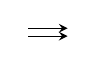
\begin{tikzpicture} \foreach \y in {0.05, 0.15} { \draw [-stealth] (0, \y) -- +(0.5, 0);} \; \end{tikzpicture}}}
\DeclareMathOperator{\leftdoublearrows} {{\; 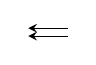
\begin{tikzpicture} \foreach \y in {0.05, 0.15} { \draw [stealth-] (0, \y) -- +(0.5, 0);} \; \end{tikzpicture}}}
\DeclareMathOperator{\righttriplearrows} {{\; 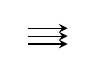
\begin{tikzpicture} \foreach \y in {0, 0.1, 0.2} { \draw [-stealth] (0, \y) -- +(0.5, 0);} \; \end{tikzpicture}}}
\DeclareMathOperator{\lefttriplearrows} {{\; 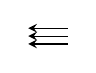
\begin{tikzpicture} \foreach \y in {0, 0.1, 0.2} { \draw [stealth-] (0, \y) -- +(0.5, 0);} \; \end{tikzpicture}}}
\DeclareMathOperator{\rightquadarrows} {{\; 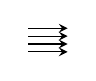
\begin{tikzpicture} \foreach \y in {-0.05, 0.05, 0.15, 0.25} { \draw [-stealth] (0, \y) -- +(0.5, 0);} \; \end{tikzpicture}}}
\DeclareMathOperator{\leftquadarrows} {{\; 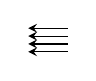
\begin{tikzpicture} \foreach \y in {-0.05, 0.05, 0.15, 0.25} { \draw [stealth-] (0, \y) -- +(0.5, 0);} \; \end{tikzpicture}}}

\newcommand{\ngon}[2][0]{
\begin{tikzpicture}[baseline=-0.5ex,scale=0.8]
\foreach \x in {1, ..., #2}
	\draw (360*\x/#2+#1:.8cm)--(360*\x/#2+#1:.5cm);
\foreach \x in {1, ..., #2}
	\draw (360*\x/#2+#1:.5cm) .. controls +(360*\x/#2+120+#1:.3cm) and +(360*\x/#2+360/#2-120+#1:.3cm) .. (360*\x/#2+360/#2+#1:.5cm);
\end{tikzpicture}
}

\newcommand{\nvertex}[2][0]{
\begin{tikzpicture}[baseline=-0.5ex,scale=0.8]
\foreach \x in {1, ..., #2}
	\draw (360*\x/#2+#1:.8cm)--(0,0);
\end{tikzpicture}
}

\newcommand{\unknot}{
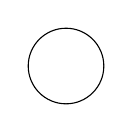
\begin{tikzpicture}[baseline=-0.5ex,scale=0.8]
  \draw (0,0) circle (.6cm);
\end{tikzpicture}
}

\newcommand{\drawI}{ 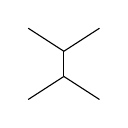
\begin{tikzpicture}[baseline=-0.5ex,scale=0.8]
 	\draw (0,.2) -- (45:.8cm);
 	\draw (0,.2) -- (135:.8cm);
	\draw (0,.2) -- (0,-.2);
 	\draw (0,-.2) -- (-45:.8cm);
 	\draw (0,-.2) -- (-135:.8cm);
\end{tikzpicture}
}

\newcommand{\drawH}{ 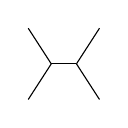
\begin{tikzpicture}[baseline=-0.5ex,rotate=90,scale=0.8]
 	\draw (0,.2) -- (45:.8cm);
 	\draw (0,.2) -- (135:.8cm);
	\draw (0,.2) -- (0,-.2);
 	\draw (0,-.2) -- (-45:.8cm);
 	\draw (0,-.2) -- (-135:.8cm);
\end{tikzpicture}}

\newcommand{\onestrandid}{\begin{tikzpicture}[baseline=-0.5ex,scale=0.8]
	\draw (-.8cm,0)--(.8cm,0);
\end{tikzpicture}}

\newcommand{\twostrandid}{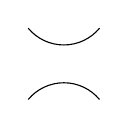
\begin{tikzpicture}[baseline=-0.5ex,scale=0.8]
	\draw (45:.8cm) to [curve through=(90:.3cm)] (135:.8cm);
	\draw (-45:.8cm) to [curve through=(-90:.3cm)] (-135:.8cm);
\end{tikzpicture}}

\newcommand{\cupcap}{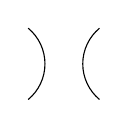
\begin{tikzpicture}[baseline=-0.5ex,rotate=90,scale=0.8]
	\draw (45:.8cm) to [curve through=(90:.3cm)] (135:.8cm);
	\draw (-45:.8cm) to [curve through=(-90:.3cm)] (-135:.8cm);
\end{tikzpicture}}

\newcommand{\symcross}{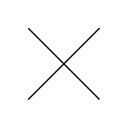
\begin{tikzpicture}[baseline=-0.5ex,scale=0.8]
	\draw (45:.8cm) -- (-135:.8cm);
	\draw (-45:.8cm) -- (135:.8cm);
\end{tikzpicture}}

\newcommand{\braidcross}{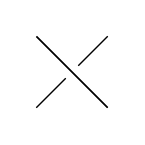
\begin{tikzpicture}[baseline=-0.5ex,scale=0.8]
	\draw (45:.8cm) -- (-135:.8cm);
	\draw[line width=1mm,white,double=black] (-45:.8cm) -- (135:.8cm);
\end{tikzpicture}}


\newcommand{\drawcrossX}{ 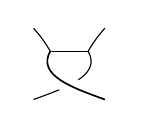
\begin{tikzpicture}[baseline=-0.5ex,scale=0.8,rotate=90]
 	\draw ([out angle=30].2,.3) .. (45:.8cm);
	\draw (.2,.3) -- (.2,-.3);
 	\draw ([out angle=-30].2,-.3) .. (-45:.8cm);
        \draw ([out angle=-150].2,-.3) ..([in angle=-70]135:.8cm);
 	\draw[line width=1mm,white,double=black]
              ([out angle=150].2,.3) .. ([in angle=70]-135:.8cm);
\end{tikzpicture}}

\newcommand{\twist}{
  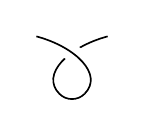
\begin{tikzpicture}[baseline=-0.5ex,scale=0.8]
    \draw[line width=1mm,white,double=black]
       ([out angle=-15]135:.8cm)..([blank=soft]-60:.4cm)..(-120:.4cm)..([in angle=-165]45:.8cm);
    \draw[line width=1mm,white,double=black,use previous Hobby path={invert soft blanks,disjoint}];
  \end{tikzpicture}}

\newcommand{\twistvertex}{
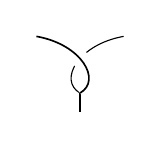
\begin{tikzpicture}[baseline=-0.5ex,scale=0.8]
  \draw (0,-0.5)--(0,-0.8);
  \draw ([out angle=-170]30:0.8cm)..([in angle=150](0,-0.5);
  \draw[line width=1mm,white,double=black]
        ([out angle=-10]150:0.8cm)..([in angle=30](0,-0.5);
\end{tikzpicture}}

\newcommand{\loopvertex}{
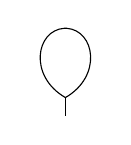
\begin{tikzpicture}[baseline=-0.5ex,scale=0.8]
  \draw (0,-0.5)--(0,-0.8);
  \draw ([out angle=150]0,-0.5)..(-0.02,0.6)..(0.02,0.6)..([in angle=30]0,-0.5);
\end{tikzpicture}
}

\newcommand{\pentagon}{
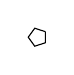
\begin{tikzpicture}[scale=.12,baseline=-2]
\draw (36:1) -- (108:1) -- (180:1) -- (252:1) -- (-36:1) -- (36:1);
\end{tikzpicture}
}

\newcommand{\psq}{
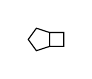
\begin{tikzpicture}[scale=.15,baseline=-2]
\draw (36:1) -- (108:1) -- (180:1) -- (252:1) -- (-36:1) -- (36:1) -- +(1.2,0) -- ($(-36:1)+(1.2,0)$) -- (-36:1);
\end{tikzpicture}
}

\newcommand{\sqsq}{
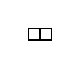
\begin{tikzpicture}[scale=.15]
\draw (0,0) -- (2,0) -- (2,1) -- (0,1) -- cycle (1,0) -- (1,1);
\end{tikzpicture}
}


\begin{document}
\title{Towards the quantum exceptional series}

\author[Morrison]{Scott Morrison}
\address{Mathematical Sciences Institute, Australian National University}
\email{scott.morrison@anu.edu.au}

\author[Snyder]{Noah Snyder}
\address{Bloomington, Indiana, USA}
\email{nsnyder1@indiana.edu}

\author[Thurston]{Dylan~P.~Thurston}
\address{Bloomington, Indiana, USA}
\email{dpthurst@indiana.edu}

\begin{abstract}
  We find a single two-parameter skein relation on trivalent graphs,
  the \emph{quantum exceptional relation}, that specializes to a skein
  relation associated to each exceptional Lie algebra (in the adjoint
  representation). If a slight
  strengthening of Deligne's conjecture on the existence of a
  (classical) exceptional series is true, then this relation
  holds for a new two-variable quantum exceptional polynomial, at
  least as a power series near $q=1$. The
  single quantum exceptional relation implies both the
  Jacobi relation (true for every Lie algebra) and
  the Vogel relation holding for the exceptional series.

  We find a conjectural basis for the space of diagrams with $n$ loose
  ends modulo the quantum exceptional relation for $n \le 7$, with
  dimensions agreeing with the classical computations, and compute
  the matrix of inner products. \nn{(Dimensions of idempotents?)}
  We use the
  skein relation to compute the conjectural quantum exceptional
  polynomial for many knots, in particular
  determining (unconditionally) the values of the quantum polynomials
  for the exceptional Lie algebras on
  these knots. The knots we can compute for include all knots with up
  to 11 (12?) crossings.
\end{abstract}

%\subjclass[2000]{Primary xxx; Secondary xxx}
%\keywords{}

\maketitle

\tableofcontents

A proposed new outline:
\begin{enumerate}
\item Introduction
\begin{enumerate}
\item Two-variable knot polynomials. For a two-variable knot polynomial to
exist, we first need a family of Lie algebras, and second need a coherent
quantisation of the family. We propose that this can be achieved in the 
exceptional series, and give many calculations of the conjectured knot
invariant.
\item Deligne's classical exceptional series, generators, relations, and 
conjectures.
\item The main result of this paper is a conjecture.
The quantum exceptional series, generators and relations and conjectures.
\item The rest of the paper consists of two kinds of evidence for this 
conjecture.
\begin{enumerate}
\item First, we show that the proposed description of the quantum exceptional 
series is the right one --- it is picked out as the unique braided tangle
category
with ...
\item Second, we give some weak evidence that the conjecture is viable.
\begin{enumerate}
\item We propose bases for the $n$-box spaces, $n \leq 6$ (or is it 7?), 
showing that these are linear independent, and their spans are closed under
various operations.
\item We show that these give representations of the affine $n$-strand braid 
groups, for $n \leq 6$.
\item We calculate ridiculously many two-variable knot polynomials; although 
these are conjectural, they unconditionally specialise to the correct quantum
knot polynomials for the exceptional Lie algebras.
\end{enumerate}
\item Mention the Kontsevich integral argument?
\end{enumerate}
\end{enumerate}
\item Main results
\begin{enumerate}
\item The classification statement.
\item We defer some corner cases to the end.
\item Proof of the main case.
\item Statement of the evaluation and consistency conjectures.
\item Some consequences: other relations.
\item Specializations.
  \begin{enumerate}
  \item $U_q(\fg)$ for $\fg$ in Deligne's list in the adjoint
    representation
  \item The 7-dimensional representation of $U_q(\fg_2)$
  \item $U_q(\fg)$ for $\fg$ in the $F_4$ family
    At $q=1$, these have $v^6=-1$ (since the trivalent vertex is
    symmetric). This family has only a finite number of points.
  \end{enumerate}
\end{enumerate}
\item Calculations
\begin{enumerate}
\item Heuristics for choosing bases for $n$-box spaces
\item Verifying linear independence, and invariance under operations
\item A representation of the affine 6-strand braid group
\item 2-variable polynomials for knots with Conway width at most 6.
\begin{enumerate}
\item Define Conway graph and Conway width.
\item Explain that we can calculate anything with Conway width at most 6.
\item This includes all 12-crossing knots, and all but one 12-crossing link.
\item Mention Westbury's paper, and the other paper that has done some knot
polynomial calculations.
\end{enumerate}
\item Denominators.
\item Dimensions of irreducible objects.
\end{enumerate}
\item A Kontsevich integral argument: the classical conjecture implies the
quantum conjecture.
\item Corner cases from the classification.
\end{enumerate}



\section{Introduction}
\label{sec:introduction}

There are two main 2-variable knot polynomials: the HOMFLY-PT polynomial and
the Kauffman polynomial.  The HOMFLY-PT polynomial interpolates between the
Reshetikhin--Turaev invariants of the standard representations of
$U_q(\mathfrak{gl}_n)$, while the Kauffman polynomial does the same for the
standard representations of quantum $U_q(\mathfrak{o}_n)$ (or, in a slightly
different form, the standard representations of $U_q(\mathfrak{sp}_n)$).  The
two variable nature of these knot polynomials come from the two parameters $n$
and $q$.  One can think of this process in two steps: first construct a family
of Lie algebra objects in symmetric tensor categories which interpolate
between the $\mathfrak{gl}_n$ yielding something called $\mathfrak{gl}_t$, and
second quantize these Lie algebra objects.   This quantization can be done
systematically using the Kontsevich integral, provided it converges.

Work of Deligne, Cvitanović, Vogel, Cohen-de Man, and others, can be summarized as a
conjecture that there is a third 1-parameter family of Lie algebra objects in
symmetric tensor categories, called the (classical) exceptional series.
This should interpolate between the
adjoint representations of $\mathfrak{sl}_2$, $\mathfrak{sl}_3$,
$\mathfrak{so}_8$, $\mathfrak{g}_2$, $\mathfrak{f}_4$, $\mathfrak{e}_6$,
$\mathfrak{e}_7$, and $\mathfrak{e}_8$.  If this classical exceptional family
exists, we should again expect a quantization yielding a 2-variable
exceptional knot polynomial.  In this paper we give a conjectural skein
theoretic description of this exceptional knot polynomial. In fact, we
prove that these relations must hold if the exceptional knot polynomial
exists.

We can use these skein relations to do many computations.  In
particular, we are able to calculate the value of this knot polynomial (if it
exists!) on all knots of Conway girth 6, which includes all knots of 12 or
fewer crossings.  For example, we compute the following value for the trefoil.

\nn{value of trefoil goes here}

In order to explain how we calculate these knot polynomials, let us first
recall Vogel's conjectural skein theoretic description of Deligne's classical
exceptional series.  We begin with the spherical tensor category of Jacobi
diagrams, $\mathrm{Jac}_d$.

\begin{definition}
Let $R$ be an algebra over $\mathbb{C}$, and let $d$ be an element of $R$ and $b$ an invertible element of $R$.  The objects of $\mathrm{Jac}_{R,d,b}$ are collections of $n$ points on the line and
the morphism space from $n$ to $m$ consists of $R$-linear combinations
of planar
graphs in a rectangle with $n$ boundary points on the bottom, $m$ boundary
points at the top, and consisting of trivalent vertices and $4$-valent
symmetric crossings
\DPTtodo{Expand on ``symmetric crossing''}
modulo planar isotopy, the usual Reidemeister 2 and 3
relations for a symmetric crossing, and the following circle,
lollipop, bigon, triangle,
anti-symmetry, symmetry of the Killing form, and Jacobi relations.

\begin{align}
\label{eq:classical-loop-lollipop}  \unknot \; &= d &  \loopvertex \; &=0 \\
\label{eq:classical-bigon-trigon}  \ngon{2}\; &= b \;\onestrandid  & \ngon{3}\; &= \frac{b}{2} \;\nvertex{3} \\
\label{eq:classical-symmetry-antisymmetry}   \symtwistvertex\; &= - \nvertex[-90]{3} & \symtwist\; &= \onestrandid
\end{align}
\begin{equation}
\drawI\; - \;\drawH\; + \;\drawsymcrossX\; = 0.
\label{eq:IHX}
\end{equation}
\end{definition}

By rescaling the trivalent vertex, it is easy to see that $\mathrm{Jac}_{R,d,b}$ is equivalent as a spherical tensor category to $\mathrm{Jac}_{R,d,bx^2}$ for any invertible $x$ in $R$.  In particular, if $R = \mathbb{C}$ then $\mathrm{Jac}_{R,d,b}$ does not depend on the choice of $b$.  A standard normalization is $b=6$.

If $\mathfrak{g}$ is a simple Lie algebra object in a symmetric tensor
category with dimension $d$, by the diagram calculus  the symmetric tensor
category of finite dimensional representations of $\mathfrak{g}$ is
the target of a
functor from $\mathrm{Jac}_{R,d,b}$, where we interpret each strand as a copy of
$\mathfrak{g}$, each cup or cap using the Killing form, each trivalent vertex
as the Lie bracket, and each crossing as the usual symmetric braiding.  This 
skein theory is somewhat poorly behaved since the space of $0$-boundary point
diagrams is expected to be infinite dimensional.

In addition, Cvitanović and Vogel independently observed that the
adjoint representations
of the exceptional Lie algebras satisfy another relation, the \emph{classical exceptional
relation}.


\begin{definition}
If $2+d$ is invertible in $R$, let $\mathrm{Exc}_{R,d,b}$ be symmetric tensor category which is the quotient of 
$\mathrm{Jac}_{R,d,b}$ modulo Vogel's exceptional relation.
\begin{equation}
\ngon[45]{4}\; = \frac{b}{6} \left(\;\drawI\; + \;\drawH\; \right)
 + \frac{5}{6}\frac{b^2}{2+d} \left( \;\twostrandid\; + \;\cupcap\; + \;\symcross\; \right)
\label{eq:classical-except}
\end{equation}
\end{definition}


\begin{conjecture} \label{conj:classical}
\DPTtodo{Do we have a particular finite set in mind? If so, give a
  pointer. How can the relevant polynomials involve $b$?}
So long as a certain finite set of polynomials in $d$ are invertible, the space of $n$-boundary point diagrams in $\mathrm{Exc}_{R,d,b}$  is free of finite rank over $R$ for every $n$, and the space of $0$-boundary point diagrams is rank $1$.  
\end{conjecture}

One should think of this conjecture as having two
parts: first a uniqueness conjecture saying that all the spaces are finite
dimensional and the $0$-boundary point space is at most $1$-dimensional, and
second a consistency conjecture saying that the category is nonzero.
Morally, the uniqueness conjecture says that we can evaluate complicated
diagrams, while the existence conjecture says that this evaluation is well-defined
 (i.e. independent of choices along the way). Although both conjectures
are completely open, we would expect uniqueness to be easier than existence.

The parameter $d$ is somewhat poorly behaved, and so Deligne instead
introduced a parameter $\lambda$ such that $d = -2
\frac{(\lambda+5)(6-\lambda)}{\lambda(1-\lambda)}$.  Note that
$\lambda$ and $1-\lambda$ correspond to the same $d$ and thus to the
same category.  If we normalize $b=6$ then the exceptional relation
for $\mathrm{Exc}_{R,-2
  \frac{(\lambda+5)(6-\lambda)}{\lambda(1-\lambda)},6}$ (which we
will also write $\mathrm{Exc}_{R,\lambda}$) has the following form.

\begin{equation}
\ngon[45]{4}\; = \;\drawI\; + \;\drawH\;
 - \frac{\lambda(1-\lambda)}{2} \left( \;\twostrandid\; + \;\cupcap\; + \;\symcross\; \right)
\label{eq:classical-except-2}
\end{equation}


The following corollary follows from Conjecture \ref{conj:classical}.

\begin{corollary}
If $d$ is one of $-5, -4, -3, -2, -3/2,1,2/3,1/2, 1/3, 1/5$, then the quotient of $\mathrm{Jac}_{\mathbb{C},d,b}$ by the negligible elements is equivalent to the category of representations of the trivial group, $O(1 | 2)$, $\mathrm{PSL}(2)$, $\mathrm{PSL}(3) \rtimes \mathbb{Z}/2$, $G_2$, $\mathrm{PO}(8) \rtimes \mathbb{Z}/3$, $F_4$, $E_6 \rtimes \mathbb{Z}/2$, $E_7$, and $E_8$, respectively.
\end{corollary}

\begin{conjecture}
There is a dense open subset $U \subset \mathbb{C}$ for which the idempotent completion of $\mathrm{Jac}_{\mathbb{C},d,b}$, for $d \in U$, is semisimple.
\end{conjecture}

We expect that in order for the idempotent completion to be semisimple one needs to invert infinitely many polynomials.  For example, for the idempotent completion of $\mathrm{GL}_t$ to be semisimple you need to invert $t-n$ for every positive integer $n$.


These conjectures are a restatement of the conjectures of Deligne and Cohen--De Man, and would give a construction of an
exceptional series passing through each of the exceptional Lie algebras.

The main result of this paper is a quantum version of this conjecture.  
Before stating this conjecture we fix some notation that is analogous to ``quantum
integer'' notation, adapted to a two-variable setting, but note that there is
no denominator.
\begin{align*}
[k\lambda + n] &= w^kv^n - w^{-k}v^{-n}\\
\{k\lambda + n\} &= w^k v^n + w^{-k} v^{-n} = \frac{[2k+2n]}{[k+n]}.
\end{align*}

\begin{definition}
Let  $\mathrm{QExc}_{R,v,b,\alpha}$ be the ribbon category whose objects are collections of $n$
points on a line, and whose morphisms spaces from $n$ to $m$ consist of $R$-linear
combinations planar graphs in a rectangle with $n$ boundary points on the
bottom, $m$ boundary points at the top, and consisting of trivalent vertices
and $4$-valent braided crossings modulo planar isotopy, the usual Reidemeister
2 and 3 relations for a symmetric crossing, and the following circle,
lollipop, bigon, triangle, quantum anti-symmetry, and quantum Killing
symmetry
relations.
\end{definition}

 \begin{equation}
    \label{eq:simple-rels-spec}
  \begin{aligned}
    \unknot\; &= d&\quad
    \loopvertex\;&=0\\[5pt]
      \ngon{2}\;&= b\;\onestrandid&
        \ngon[-90]{3}\; &= t\;\nvertex[-90]{3}\\[5pt]
    \twistvertex\; &= -v^{6}\;\nvertex[-90]{3}&
      \twist\; &= v^{12}\;\onestrandid
  \end{aligned}
  \end{equation}
where
\begin{align*}
  d &= -\frac{\{2\}[\lambda+5][\lambda-6]}{[\lambda][\lambda-1]}\\
  b &= \frac{\{\lambda+2\}\{\lambda-3\}[3]}{[1]}\\
  t &= \{1\}\bigl(\{1\}w^2/v + (v^4 - v^2 - 1 - v^{-2} + v^{-4}) +
      \{1\}v/w^2\bigr).
\end{align*}
To these skein relations, we add the \emph{quantum IHX relation}
\begin{equation}
v^{-3} \;
\drawcrossX
\;+ v \;
\drawI
\; -v^{-1} \;
 \drawH
\;
 - \frac{[\lambda][\lambda-1]}{[1]}
\left[\; \braidcross \;
 + v^{4}\;
\twostrandid
\; + v^{-4} \;
 \cupcap \;
 \right] = 0.\label{eq:quant-except-spec}
\end{equation}













\begin{definition}
Let \nn{name?} be the ribbon category whose objects are collections of $n$
points on a line, and whose morphisms spaces from $n$ to $m$ consist of linear
combinations planar graphs in a rectangle with $n$ boundary points on the
bottom, $m$ boundary points at the top, and consisting of trivalent vertices
and $4$-valent braided crossings modulo planar isotopy, the usual Reidemeister
2 and 3 relations for a symmetric crossing, and the following circle,
lollipop, bigon, triangle, quantum anti-symmetry, and quantum Jacobi
relations.
\end{definition}

 \begin{equation}
    \label{eq:simple-rels-spec}
  \begin{aligned}
    \unknot\; &= d&\quad
    \loopvertex\;&=0\\[5pt]
      \ngon{2}\;&= b\;\onestrandid&
        \ngon[-90]{3}\; &= t\;\nvertex[-90]{3}\\[5pt]
      \twist\; &= v^{12}\;\onestrandid&
        \twistvertex\; &= -v^{6}\;\nvertex[-90]{3}
  \end{aligned}
  \end{equation}
where
\begin{align*}
  d &= -\frac{\{2\}[\lambda+5][\lambda-6]}{[\lambda][\lambda-1]}\\
  b &= \frac{\{\lambda+2\}\{\lambda-3\}[3]}{[1]}\\
  t &= \{1\}\bigl(\{1\}w^2/v + (v^4 - v^2 - 1 - v^{-2} + v^{-4}) +
      \{1\}v/w^2\bigr).
\end{align*}
To these skein relations, we add the \emph{quantum IHX relation}
\begin{equation}
v^{-3} \;
\drawcrossX
\;+ v \;
\drawI
\; -v^{-1} \;
 \drawH
\;
 - \frac{[\lambda][\lambda-1]}{[1]}
\left[\; \braidcross \;
 + v^{4}\;
\twostrandid
\; + v^{-4} \;
 \cupcap \;
 \right] = 0.\label{eq:quant-except-spec}
\end{equation}

We conjecture that the skein relations above suffice to evaluate
uniquely every framed knotted trivalent graph. In fact we split the
conjecture up into different parts.

\DPTtodo{Introduced some placeholder terminology here so I could state
  the conjectures more precisely. Feel free to change it.}
Let $R$ be the ring $\QQ[v,w,v - v^{-1},w - w^{-1}, w/v - v/w]$, that
is, the minimal ring for which all of the denominators in the skein
relations are defined. Let $\Skq{n,m}$ be the \emph{skein algebra vector space}
of framed, embedded trivalent $(n,m)$ tangles modulo the
local skein relations in \eqref{eq:simple-rels-spec}
and~\eqref{eq:quant-except-spec}. The different vector spaces
$\Skq{n,m}$ combine into a category $\Skqcat$ where the objects are
integers and the morphisms from $n$ to $m$ are elements of $\Skq{n,m}$.

\begin{conjecture}[Quantum consistency]
  \label{conj:quant-consist}
  There is a category $\mathsf{QExcept}$ where the objects are
  integers and morphisms are finite-dimensional, free $R$-modules, and
  a functor $\eval$ from $\Skqcat$ to $M_n$, that is the identity on
  objects and surjective on morphisms after extending scalars to
  $\QQ(v,w)$. Furthermore, $\mathsf{QExcept}(n,m)$ has dimension
  $1,\allowbreak0,\allowbreak1,\allowbreak1,\allowbreak5,\allowbreak16,\allowbreak80$
  for $n+m=0,1,2,3,4,5,6$, respectively, and $\eval$ takes a single
  strand and a trivalent vertex to generators of the respective
  morphism spaces.
\end{conjecture}

\DPTtodo{Is this too weak? To derive square reduction, we do assume
  something more about the denominators, so we probably do need to
  extend scalars at least a little. Would be nice to have a version of
  sufficiency that doesn't assume consistency}
\begin{conjecture}[Quantum sufficiency]
  \label{conj:quant-suffic}
  After extending scalars to $\QQ(v,w)$, the functor $\eval$
  conjectured above is injective on each morphism space. In
  particular, these relations suffice to evaluate any closed framed
  trivalent graph to a rational function in $v$ and~$w$.
\end{conjecture}

The relations above are quite general. With some mild assumptions on the base
ring, any skein theory where the $n$-box space has dimension at most
$1,0,1,1,5$ for $n=0,1,2,3,4$ satisfies a version of relation~\eqref{eq
:quant-except-spec}. See Theorem~\ref{thm:quant-except} in
Section~\ref{sec:relation} for a precise statement.







 

Note that unconditionally, these 2-variable knot polynomials must specialize
at particular values of $w$ to give the quantum invariants of the adjoint
representations of the actual Lie algebras.  To our knowledge these are the
first calculations of the quantum knot polynomials of large knots for say
$\mathfrak{e}_8$, and they are much more efficient than doing the calculations
directly in $U_q(\mathfrak{e}_8)$.  Also unconditionally we show that our
skein relations give a well-defined $80$-dimensional representation of the
affine $6$-strand braid group.  Using our skein relations, we also compute the
quantum versions of Cohen--De Man's formulas for the dimensions of the objects
appearing in the third tensor power of adjoint representation in the
exceptional series.

Finally, we consider what happens when $v$ specializes to a $12$th or $10$th
root of unity, where some of our skein relations have vanishing denominators.
It turns out that there is still a natural way to define these
specializations, and they recover some interesting examples including the
classical exceptional series, the classical $\mathfrak{g}_2$ series, the
classical $\mathfrak{f}_4$ series, Deligne's interpolated symmetric group
categories, and a possible new example related to the ABA free product from
\cite{???}.


\section{Main results}

\section{Calculations}
\label{sec:calculations}
\newcommand{\V}{\mathcal{P}}

\subsection{Heuristics for bases}
\section{Candidate bases}
We now consider two candidates bases, $\cB^{\text{braided}}$ and $\cB^{\text
{planar}}$ for each of the spaces $\cP_n$, for $n = 2,3,4,5,6$.
At this point we can only give heuristics for choosing these sets of diagrams;
in the next section we will establish that they are linearly independent, but
it is beyond the scope of this paper to show that they span --- this is
probably at least as hard as showing that the quantum exceptional relation
suffices to evaluate all closed diagrams. Nevertheless they have the expected
sizes, following Cohen--de-Man's claim that the invariant spaces for
$\mathfrak{f}_4$ do not degenerate up to $\cP_6$:
\[
\begin{tabular}{rr}
  \toprule
  $n$ & $\dim \Hom_{\mathfrak{f}_4} (1 \to \mathfrak{f}_4^{\otimes n})$ \\
  \midrule
  0 & 1 \\ 1 & 0 \\ 2 & 1 \\ 3 & 1 \\ 4 & 5 \\ 5 & 16 \\
  6 & 80 \\ 7 & 436 \\ 8 & 2891 \\ 9 & 22248 \\ 10 & $\ge 198774$ \\
  \bottomrule
\end{tabular}
\]

\nn{Some discussion of the heuristic for choosing these bases.}

\newcommand{\diagram}[2]{\mathfig{#1}{graphs/urn:sha1:#2.pdf}}

In order to write our proposed bases compactly, we introduce the following
notations: $D_{*k}$ denotes the diagram $D$ along with all $k$ of its
inequivalent rotations (when $D$ has $n$ boundary points, $k$ divides $n$),
and $D_{*k!}$ denotes the diagram $D$ along with the first $k$ of its
counterclockwise rotations, even though these do not exhaust all of the
inequivalent rotations.

\DPTtodo{The graphs look good, but the lines should be thicker at this
size}
We define them as follows:
\begin{align*}
\cB^{\text{braided}}_0 & = \cB^{\text{planar}}_0 = \left\{ \diagram
{0.1}{8093b057e0fa058603d83e620c4490c7774731e}_{*1}\right\} &
\cB^{\text{braided}}_1 & = \cB^{\text{planar}}_1 = \Bigg\{ \quad \Bigg\} \\
\cB^{\text{braided}}_2 & = \cB^{\text{planar}}_2 = \left\{ \diagram
{0.1}{1f3bf4bb66a4388fb2984eb673be4539182b0256}_{*1} \right\} &
\cB^{\text{braided}}_3 & = \cB^{\text{planar}}_3 = \left\{ \diagram
{0.1}{a7ce858dc75f8bbfee5e1b9837d3d13991f48637}_{*1} \right\}
\end{align*} 
\begin{align*}
\cB^{\text{braided}}_4 & = \left\{ 
  \diagram{0.1}{34a876bb5dae61c3ae047f077a51c37b92ee0789}_{*2},
  \diagram{0.1}{a3a76e07ebde41b851fc63a935929666fca9dcd6}_{*2},
  \diagram{0.1}{d4f429174ebdeb2777a6e5c1f7d726caca7350cd}_{*1!}
  \right\} \\
\cB^{\text{braided}}_5 & = \left\{ 
  \diagram{0.1}{e55fafbd03afa4f32c7a584ff8fc14d93149f64e}_{*5},
  \diagram{0.1}{7852166906e0c69e28a717a274dd63ebb2dd14bf}_{*5},
  \diagram{0.1}{25d22603781a5a699a84b26b177c0c228abe0e7a}_{*5},
  \diagram{0.1}{6c16eee9baf0b996fa06ef435e4f0229abade522}_{*1!}
  \right\} \\
\cB^{\text{braided}}_6 & = \Bigg\{ 
  \diagram{0.1}{a906b4797b1a0522970b8c97cdb5415a37a14d50}_{*2},
  \diagram{0.1}{1d5fda6573f6e14e019449f842ce86389a666ef3}_{*3},
  \diagram{0.1}{e9f2d2b49d091b0935f5fbd5087a91496a8aea65}_{*6},
  \diagram{0.1}{ae1c9ad2880e168051d75739ff9ac571f47d5418}_{*3},
  \diagram{0.1}{435c40660d57b8d767e9699896b711416756716b}_{*1!},
  \diagram{0.1}{3b78ddd6226e5dcf91391aad721c40afb6d9dce7}_{*3}, \displaybreak
  [1] \\
  & \qquad
  \diagram{0.1}{c46af9af2acf5cc00e83232f57fbe67cc3a43b22}_{*6},
  \diagram{0.1}{6b9f6a4077a98d93b7ef68d31d192895cca8de84}_{*6},
  \diagram{0.1}{562a17e80676bec7f61ae4cf18c3cc7c22b9f761}_{*6},
  \diagram{0.1}{2e79238a0fa16c77b7e1b0762abafe754d1f7725}_{*1!}
  \diagram{0.1}{392d6cefb5870ced299b7f7140b7253a42e32c47}_{*6},
  \diagram{0.1}{6457494dd06c026dc17137d37534cc940ba96844}_{*6}, \displaybreak[1]
  \\
  & \qquad
  \diagram{0.1}{8b6e9125e28b6e81350cac1329d9e353792cf06}_{*3!},
  \diagram{0.1}{3b74991ad2c977fa674f4891439a048a05ac0525}_{*3},
  \diagram{0.1}{1baad19a7b800a28edd9aa033244492c73330c5b}_{*3},
  \diagram{0.1}{11a1b489797895c39addff508158f439338f2bd8}_{*3},
  \diagram{0.1}{6aaaa92365996498480cfebe7eeb211bb34dca33}_{*6},
  \diagram{0.1}{82157c05fd8fcf68cf7cd7327cbcee5b7bd885a0}_{*2}, \displaybreak
  [1] \\
  & \qquad
  \diagram{0.1}{8dfbd4e54baa5d5755c7a7cef5ae974c6a737cac}_{*6},
  \diagram{0.1}{8a27a57e82333b072ffb4d5b78de022da5c0852b}_{*4!},
  \diagram{0.1}{88b8c27ab39d49cf9e9fdf6be821e0d1c86a5c31}_{*1}
\Bigg\}
\end{align*}
In most of the cases above where we only take some of the rotations of a given diagram, it is because the other rotations
are already isotopic (using 3-dimensional isotopies) to the chosen ones. The exception is that we only take 4 out of the 6 possible rotations of \diagram{0.1}{8a27a57e82333b072ffb4d5b78de022da5c0852b}. This will \nn{probably} be discussed below.

\begin{align*}
\cB^{\text{planar}}_4 & = \left\{ 
  \diagram{0.1}{34a876bb5dae61c3ae047f077a51c37b92ee0789}_{*2},
  \diagram{0.1}{a3a76e07ebde41b851fc63a935929666fca9dcd6}_{*2},
  \diagram{0.1}{ac38f78879901186d72dd46debb629071d8a75cc}_{*1}
  \right\} \\
\cB^{\text{planar}}_5 & = \left\{ 
  \diagram{0.1}{e55fafbd03afa4f32c7a584ff8fc14d93149f64e}_{*5},
  \diagram{0.1}{25d22603781a5a699a84b26b177c0c228abe0e7a}_{*5},
\diagram{0.1}{175489e116757578e7d6a10f33f29bd527db673c}_{*1},
\diagram{0.1}{fcc4cb12bd0293b0149f2355e09590e48a13cec3}_{*5}
  \right\} \\
\cB^{\text{planar}}_6 & = \Bigg\{ 
  \diagram{0.1}{a906b4797b1a0522970b8c97cdb5415a37a14d50}_{*2},
  \diagram{0.1}{1d5fda6573f6e14e019449f842ce86389a666ef3}_{*3},
  \diagram{0.1}{51e3597810ca80c60ccbf5ca773dc5f60cc05c26}_{*6},
  \diagram{0.1}{760566cf41c94808243c3091c5f724575b58def2}_{*6},
  \diagram{0.1}{36f1b77eb343f84d3afe9767721856dae4fad1b}_{*3},
  \diagram{0.1}{7faa515ce21febe73dc79066d0a32573cf6951a8}_{*3},
  \displaybreak
  [1] \\
  & \qquad 
  \diagram{0.1}{1baad19a7b800a28edd9aa033244492c73330c5b}_{*3},
  \diagram{0.1}{2ea46d95045afa05d7bd0c8f2dc292ea8d6b000b}_{*3},
  \diagram{0.1}{f357e0b86229ce63736f2ab08989fc2a2f1db2f6}_{*2},
  \diagram{0.1}{d0933ddaf142ecb016df91e1cc0762ab4cc30985}_{*6},
  \diagram{0.1}{a15b7af68d41b9e913156373e080ad2096b76fe}_{*3},
  \diagram{0.1}{cf51f65ba0c14cf15e713f6b099ed1e838e8b36b}_{*6}, \displaybreak
  [1] \\
  & \qquad 
  \diagram{0.1}{c149b820be2b7d1e7c4b136864ecf03d6d48513c}_{*6},
  \diagram{0.1}{e2072b35dc85bb5c685bc5a889493ee86bf3da8d}_{*6},
  \diagram{0.1}{63ea103b950fa114bda8149d575a29b8eaf74920}_{*6},
  \diagram{0.1}{7de6a0854fa495f044e12f0708481932e9cb121e}_{*1},
  \diagram{0.1}{49bc9767ee6402dfea4c3919f407e7a9dc9d8b59}_{*3},
  \diagram{0.1}{6a3eb98050b8a853009b33fa4bddd634b51b0efd}_{*4!}, \displaybreak
  [1] \\
  & \qquad 
  \diagram{0.1}{b849c60b70156f6044cc8c10b49bd07cd358cde7}_{*3!}, 
  \diagram{0.1}{34fabf27c9ebd1f6ece3151ab5f9cde18b1ca09b}_{*1!},
  \diagram{0.1}{5004f6fa7f2aa5d72b882308ff24d97dcd8aa047}_{*1!}
\Bigg\} 
\end{align*}
\nn{Is this right? What happens to the pentapent \diagram{0.1}{55f53ebaabfb09b3d4727e4b45c3637b0ed8f84c}? What about \diagram{0.1}{c44c9c3e568ce2218151df6d19f09681f6a6e4d8}?}


\subsection{Linear independence}
We first check that these bases are linearly independent. 
We have a pairing $\langle - , - \rangle: \V_n \otimes \V_n \to \V_0$ defined
by 
\[
  \langle x, y \rangle =
  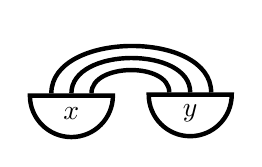
\begin{tikzpicture}[baseline, ultra thick]
    \node[draw, shape=semicircle, shape border rotate=180, minimum size=1.5em] (x) {$x$};
    \node[draw, shape=semicircle, shape border rotate=180, minimum size=1.5em, right=0.5cm of x] (y) {$y$};
    \draw (x.90) to[in=90, out=90] (y.90);
    \draw (x.135) to[in=90, out=90] (y.45);
    \draw (x.45) to[in=90, out=90] (y.135);
  \end{tikzpicture}
\]
and for many (conjecturally all) closed diagrams diagrams in $\V_0$ we can use
the relations
to evaluate to a rational function in \(\QQ(v,w)\). Of course, our basis is
far from orthonormal with respect to this pairing!

We first look at the braided bases described above, and find that, up to $n=6$, we can evaluate all matrix entries of $M_n =
\left(\langle e_i, e_j \rangle\right)_{i,j}$. We can then calculate the
determinants of these matrices, obtaining
%% These are calculated in determinants-of-inner-products.nb
\begin{align*}
\det M_3 & = - \frac{
	           \{2\} [\lambda + 5] [\lambda - 6]
             }{
               [\lambda] [\lambda - 1]
             } \\
% -((brk[0, 1] brk[0, 4]^5 brk[0, 5]^3 brk[0, 6]^4 brk[1, -6]^5 brk[
%       1, -4]^2 brk[1, -3] brk[1, 2] brk[1, 3]^2 brk[1, 5]^5 brk[
%       3, -6] brk[3, 3])/(brk[0, 2]^7 brk[0, 3]^4 brk[1, -2] brk[
%       1, -1]^8 brk[1, 0]^8 brk[1, 1] brk[2, -6] brk[2, 4]))
\det M_4 & = \frac{
              [1] [4]^5 [5]^3 [6]^4 [\lambda - 6]^5 [\lambda - 4]^2 [\lambda - 3] [\lambda + 2]
              [\lambda + 3]^2 [\lambda + 5]^5 [3\lambda - 6] [3\lambda + 3]
             }{
              [2]^7 [3]^4 [\lambda - 2] [\lambda - 1]^8 [\lambda]^8 [\lambda + 1]
              [2 \lambda - 6] [2\lambda + 4]
             } \\
% -((brk[0, 1]^7 brk[0, 4]^16 brk[0, 5]^13 brk[0, 6]^20 brk[
%       1, -6]^16 brk[1, -4]^10 brk[1, -3]^12 brk[1, 2]^12 brk[1, 
%       3]^10 brk[1, 5]^16 brk[3, -6]^6 brk[3, 3]^6 brk[4, -6] brk[4, 
%       2])/(v^2 brk[0, 2]^24 brk[0, 3]^32 brk[1, -2]^6 brk[
%       1, -1]^26 brk[1, 0]^26 brk[1, 1]^6 brk[2, -6]^12 brk[2, -3] brk[
%       2, 1] brk[2, 4]^12))
\det M_5 & = 
             \frac{
              [1]^7 [4]^{16} [5]^{13} [6]^{20} [\lambda - 6]^{16} [\lambda - 4]^{10} 
              [\lambda - 3]^{12} [\lambda + 2]^{12}
              [\lambda + 3]^{10} [\lambda + 5]^{16} [3\lambda - 6]^6 [3\lambda + 3]^6
              [4 \lambda - 6] [4\lambda + 2]
             }{
              v^2 [2]^{24} [3]^{32} [\lambda - 2]^{6} [\lambda - 1]^{26} [\lambda]^{26} [\lambda + 1]^6
              [2 \lambda - 6]^{12} [2\lambda - 3] [2\lambda + 1] [2\lambda + 4]^{12}
             } \\
\det M_6 & = \frac{
              -v^{12} [1]^{67} [4]^{80} [5]^{75} [6]^{165} [\lambda - 6]^{80} [\lambda - 5]^{15} [\lambda - 4]^{65} [\lambda - 3]^{112} [\lambda + 3]^{65} [\lambda + 4]^{15} [\lambda + 5]^{80} [2 \lambda - 4]^5 [2\lambda + 2]^5 [3\lambda - 6]^{45} [3\lambda + 3]^{45} [4 \lambda - 6]^{10} [4\lambda + 2]^{10} [5\lambda - 6] [5\lambda + 1]
             }{
               [2]^{151} [3]^{268} [\lambda - 2]^{50} [\lambda - 1]^{150} [\lambda]^{150} [\lambda + 1]^{50} [2\lambda - 6]^{107} [2\lambda - 3]^{10} [2\lambda + 1]^{10} [2\lambda + 4]^{107}
             }.
\end{align*}



In particular, we see that $\det M_4$ vanishes when $v^k = 1$ for $k=1,2,4,5,8,10$, or $12$, or when $w = \pm v^k$ for $k=-5,-3,4,6$, or when $v^4 \pm v^2 w + w^2 = 0$ (equivalently, $w = \zeta v^{-1}$ for $\zeta$ a primitive 3rd or 6th root of unity) or $1 \pm v w + v^2 w^2 = 0$ (equivalently, $w = \zeta v^2$ for $\zeta$ a primitive 3rd or 6th root of unity). Then, $\det M_5$ vanishes at all the same places, and additionally at $v^6 + w^4 = 0$ and $1 + v^2 w^4 = 0$. \nn{These are exactly the curves corresponding for quantum $E_6$.}
Finally $\det M_6$ vanishes everywhere $\det M_5$ does, and also at $w = \pm v^k$ for $k=-4,-2,3,5$, $w = \pm i v^k$ for $k=-1,2$, $v = \pm w^{-5}$ and $w^5 \pm v^6 = 0$.

In fact, the components of $\det M_4 = 0$ are explained by smaller categories which we already know about, or degenerate cases.
\nn{appropriate reference elsewhere in the paper for the $v^k = 1$ cases}
At $w = \pm v^{-5}$ and $w = \pm v^6$, we see that $d=0$, so any quotient would be degenerate. At $w = \pm v^{-3}$ and $w = \pm v^4$, we recover the $SO(3)_q$ categories \nn{details?}. At $w = \zeta v^2$, with $\zeta$ a primitive 3rd or 6th root, we obtain $(G_2)_q$ \nn{details}. \nn{What about $w = \zeta v^{-1}$?}

Although it may appear that new factors are appearing in the
denominators as we look at $\det M_3, \det M_4, \det M_5, $ and $\det
M_6$, one should recall that the bracket polynomials $[a \lambda + b]$
are not generally irreducible. \nn{Does ``irreducible'' make sense?
  $\QQ[v\pm 1, w \pm 1]$ is not a UFD, right?} The
irreducible factors appearing in the denominator after cancellation
remain the denominators \nn{already} introduced: $\det M_4$ has poles
at $w=\pm1, v=\pm w, v^6+w^2 = 0$, and $1+v^4w^2 = 0$,
then $\det M_5$ has additional poles at $w=0, 1\pm v + v^2 = 0$, and $\det M_6$
has a pole at $v = \pm 1$.


\subsection{Matrices for operations}
In this section, we obtain matrices for the braiding and rotation operators on
 $\V_n$, `relative to' $\cB^{\text{braided}}$ described above.
We have to be careful here, as we don't know that $\cB^{\text{braided}}$
actually spans $\V_n$, or even that the braiding and rotation operators map
the span of $\cB^{\text{braided}}$ to itself.

The second of these questions is relatively tractable; it would just be a
matter of applying a braiding or rotation to each element, and showing that it
is possible to use the relations to rewrite the result as a linear combination
of elements of $\cV^{\text{braided}}$. We take a slightly different approach,
computing the matrix which \emph{would} be associated to each of the
operations \emph{if} $\cB^{\text{braided}}$ really were a basis, and then
verifying that these matrices satisfy the expected properties.


Now, given an operator $T: \V_n \to \V_m$, if the $\cB^{\text{braided}}_n$
are bases, the associated matrix for $T$ would be $AM_m^{-1}$, where
$A = \left(\langle T e_i, e_j \rangle\right)_{i,j}$.
Rather unfortunately inverting the matrix $M_6$ is computationally
infeasible. (Recall that arithmetic over $\QQ(v,w)$ may be quite inefficient!)

We find, nevertheless, that for $T$ any of 
\begin{align*}
  (\rho_n : \V_n \to \V_n) & = 
    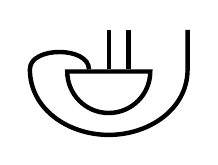
\begin{tikzpicture}[baseline, ultra thick]
      \node[draw, shape=semicircle, shape border rotate=180, minimum size=1.5em] (x) {};
      \draw (x.90) -- ++(0,0.5);
      \draw (x.45) -- ++(0,0.5);
      \draw (x.135) to[in=90, out=90] ++(-0.75,0) 
                     to[in=180,out=-90] ($(x.-90)+(0,-0.25)$) 
                     to[out=0,in=-90] ($(x.45)+(0.75,0)$)
                     -- ++(0,0.5);
    \end{tikzpicture} &
  (\beta_n : \V_n \to \V_n) & = 
    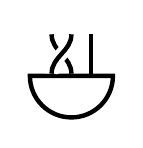
\begin{tikzpicture}[baseline, ultra thick]
      \node[draw, shape=semicircle, shape border rotate=180, minimum size=1.5em] (x) {};
      \draw (x.45) -- ++(0,0.5);
      \draw (x.90) to[out=90,in=-90] ($(x.135)+(0,0.5)$);
      \draw[knot] (x.135) to[out=90,in=-90] ($(x.90)+(0,0.5)$);
    \end{tikzpicture} 
  \displaybreak[1] \\
  (\cap_n : \V_n \to \V_{n-2}) & = 
    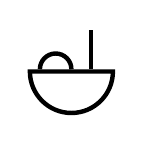
\begin{tikzpicture}[baseline, ultra thick]
      \node[draw, shape=semicircle, shape border rotate=180, minimum size=1.5em] (x) {};
      \draw (x.45) -- ++(0,0.5);
      \draw (x.90) arc (0:180:0.2);
    \end{tikzpicture}
  &
  (\cup_{n-2} : \V_{n-2} \to \V_{n}) & = 
    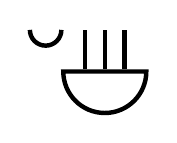
\begin{tikzpicture}[baseline, ultra thick]
      \node[draw, shape=semicircle, shape border rotate=180, minimum size=1.5em] (x) {};
      \draw (x.90) -- ++(0,0.5);
      \draw (x.45) -- ++(0,0.5);
      \draw (x.135) -- ++(0,0.5);
      \draw ($(x.135)+(0,0.5)+(-0.3,0)$) arc (0:-180:0.2);
    \end{tikzpicture}
  \displaybreak[1] \\
  (\fork_{n-1} : \V_{n-1} \to \V_{n}) & = 
    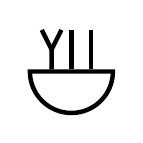
\begin{tikzpicture}[baseline, ultra thick]
      \node[draw, shape=semicircle, shape border rotate=180, minimum size=1.5em] (x) {};
      \draw (x.90) -- ++(0,0.5);
      \draw (x.45) -- ++(0,0.5);
      \draw (x.135) -- ++(0,0.25) -- ++(0.125,0.25);
      \draw    ($(x.135)+(0,0.25)$) -- ++(-0.125,0.25);
    \end{tikzpicture}
  &
  (\fuse_n : \V_n \to \V_{n-1}) & = 
    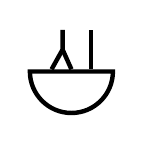
\begin{tikzpicture}[baseline, ultra thick]
      \node[draw, shape=semicircle, shape border rotate=180, minimum size=1.5em] (x) {};
      \draw (x.45) -- ++(0,0.5);
      \draw (x.90) -- ($(x.114)+(0,0.25)$);
      \draw (x.135) -- ($(x.114)+(0,0.25)$) -- ++(0,0.25);
    \end{tikzpicture}
  \\
  (H_n : \V_n \to \V_n) & = 
    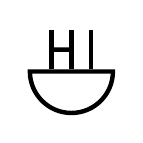
\begin{tikzpicture}[baseline, ultra thick]
      \node[draw, shape=semicircle, shape border rotate=180, minimum size=1.5em] (x) {};
      \draw (x.45) -- ++(0,0.5);
      \draw (x.90) -- ++(0,0.5);
      \draw (x.135) -- ++(0,0.5);
      \draw ($(x.90)+(0,0.25)$) -- ($(x.135)+(0,0.25)$);
    \end{tikzpicture}
\end{align*}
with $n \leq 6$,
we can evaluate all of the matrix entries of $A$ as rational functions.
(Even though $H_n = \rho_{n}^{-1} \fuse_n \rho_{n+1} \fork_n$, we can not
use this to compute $H_6$ as we would need to know $\rho_7$ and $\fuse_7$.)

Even though directly inverting $M$ is infeasible, we find that we can
calculate the product $A M^{-1}$ in each case. (Nevertheless this remains a
difficult calculation ---  we use some tricks, calculating the product at
various specialisations of the variables and then using interpolation, finally
verifying our answer by multiplying by $M$.)

Explicit matrices are available with the {\tt arXiv} sources of this article, 
as the files $$\text{{\small\tt matrices/n-box-OP-matrix.m}},$$ where $n \leq 6$, and {\tt OP}
is one of {\tt rotation},
{\tt braiding}, {\tt inverse-braiding}, {\tt cup}, {\tt cap}, {\tt fork}, {\tt
fuse}, {\tt H}. 
The matrices are written in terms of the variables $d, v$. 


\subsection{Representations of braid groups}
The affine $n$-strand braid group has generators $\rho$ and $\beta$, with
relations $\rho^n = 1$, $\beta \rho^\pm \beta \rho^\mp \beta = \rho^\pm
\beta \rho^\mp \beta \rho^\pm
\beta \rho^\mp$, and $\beta \rho^i \beta \rho^{-i} = \rho^i \beta \rho^
{-i} \beta$ for all $i = 2, \ldots, n-2$.

At this point, we may verify that the matrices $\rho = \rho_n$ and $\beta =
\beta_n$ provide a representation of the affine $n$-strand braid group merely by multiplying out the matrices. 

\begin{lemma}
The matrices described in the previous section give a representation of the affine $n$-strand braid group for $3 \leq n \leq 6$.
\end{lemma}


\subsection{A 2-variable link polynomial}

\subsubsection{Limited planar operations}
Thinking of the vector spaces $\V_n$ as forming a planar algebra, 
at this point we have limited access to the full set of operations indexed by
planar tangles. We have computed above
$\cap_n : \V_n \to \V_{n-2}$, 
$\cup_{n-2} : \V_{n-2} \to V_n$, and
$\rho_n: \V_n \to \V_n$ for $n \leq 6$. We can also find
\begin{align*}
(m_{4,4,2} : \V_4 \otimes \V_4 \to \V_4) & = 
  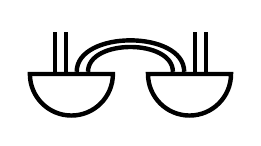
\begin{tikzpicture}[baseline, ultra thick]
    \node[draw, shape=semicircle, shape border rotate=180, minimum size=1.5em] (x) at (0,0) {};
    \node[draw, shape=semicircle, shape border rotate=180, minimum size=1.5em] (y) at (1.5,0) {};
    \draw (x.130) -- +(0,0.5);
    \draw (x.105) -- +(0,0.5);
    \draw (x.75) to[out=90,in=90] (y.105);
    \draw (x.50) to[out=90,in=90] (y.130);
    \draw (y.75) -- +(0,0.5);
    \draw (y.50) -- +(0,0.5);
  \end{tikzpicture}
 \displaybreak[1] \\
(m_{4,6,2} : \V_4 \otimes \V_6 \to \V_6) & = 
  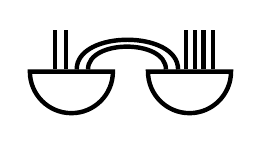
\begin{tikzpicture}[baseline, ultra thick]
    \node[draw, shape=semicircle, shape border rotate=180, minimum size=1.5em] (x) at (0,0) {};
    \node[draw, shape=semicircle, shape border rotate=180, minimum size=1.5em] (y) at (1.5,0) {};
    \draw (x.130) -- +(0,0.5);
    \draw (x.105) -- +(0,0.5);
    \draw (x.75) to[out=90,in=90] (y.120);
    \draw (x.50) to[out=90,in=90] (y.140);
    \draw (y.100) -- +(0,0.5);
    \draw (y.75) -- +(0,0.5);
    \draw (y.55) -- +(0,0.5);
    \draw (y.40) -- +(0,0.5);
  \end{tikzpicture}
 \displaybreak[1] \\
\intertext{and}
(m_{4,4,1} : \V_4 \otimes \V_4 \to \V_6) & = 
  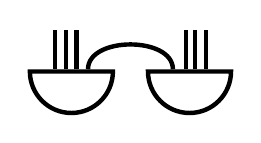
\begin{tikzpicture}[baseline, ultra thick]
    \node[draw, shape=semicircle, shape border rotate=180, minimum size=1.5em] (x) at (0,0) {};
    \node[draw, shape=semicircle, shape border rotate=180, minimum size=1.5em] (y) at (1.5,0) {};
    \draw (x.130) -- +(0,0.5);
    \draw (x.105) -- +(0,0.5);
    \draw (x.75) -- +(0,0.5);
    \draw (x.50) to[out=90,in=90] (y.130);
    \draw (y.100) -- +(0,0.5);
    \draw (y.75) -- +(0,0.5);
    \draw (y.50) -- +(0,0.5);
  \end{tikzpicture}
\end{align*}
 as follows.

Recall that our chosen basis for $\V_4$ is
\[
  \left(
    \tikz[baseline=-7, ultra thick]{\draw(0,0) arc (-180:0:0.2); \draw(0.6,0) arc(-180:0:0.2);},
    \tikz[baseline=-7, ultra thick]{\draw(0,0) arc (-180:0:0.4); \draw(0.2,0) arc(-180:0:0.2);},
    \tikz[baseline=-7, ultra thick]{\draw(0,0) arc (-180:0:0.2); \draw(0.6,0) arc(-180:0:0.2);
                       \draw(0.2,-0.2) arc (-180:0:0.3);},
    \tikz[baseline=-7, ultra thick]{\draw(0,0) arc (-180:0:0.4); \draw(0.2,0) arc(-180:0:0.2);
                       \draw(0.4,-0.4) -- (0.4,-0.2);},
    \tikz[baseline=-7, ultra thick]{\draw(0,0) arc (-180:0:0.3); \draw[knot] (0.3,0) arc (-180:0:0.3);}
  \right)
\]
Expressed in our chosen bases, we then have 
\begin{align*}
  m_{4,n,2}((x_1, x_2, x_3, x_4, x_5) \otimes y)
    & = x_1 \cup_{n-2}\cap_n y \\
      & \quad + x_2 y \\
      & \quad + x_3 \fork_{n-1}\fuse_n y \\
      & \quad + x_4 H_n y \\
      & \quad + x_5 \beta y.
\end{align*}
Finally, we can write $m_{4,4,1}$ in terms of the other operations, e.g.
as
$$
 m_{4,4,1}(x \otimes y) = m_{4,6,2}(x \otimes \rho_6^{-1} (\cup_4 (\rho_4(y)))
 = 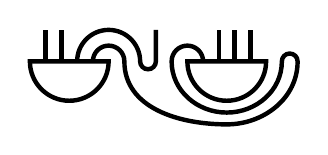
\begin{tikzpicture}[baseline, ultra thick]
     \draw (0,0) arc (-180:0:0.5) -- cycle;
     \draw (2,0) arc (-180:0:0.5) -- cycle;
     \draw (2.2,0) arc (0:180:0.2) to[out=-90,in=180] (2.5,-0.65) to[out=0,in=-90] (3.2,0) arc (180:0:0.1) to[out=-90,in=0] (2.5,-0.8) to[out=180,in=-90] (1.2,0) arc (0:180:0.2);
     \draw (0.6,0) arc (180:0:0.4) arc (-180:0:0.1) -- +(0,0.4);
     \draw (0.2,0) -- +(0,0.4);
     \draw (0.4,0) -- +(0,0.4);
     \draw (2.4,0) -- +(0,0.4);
     \draw (2.6,0) -- +(0,0.4);
     \draw (2.8,0) -- +(0,0.4);
   \end{tikzpicture}
$$ 

\subsubsection{Conway girth}
Typically, we may choose to think about a diagrammatically defined tangle 
invariant as a morphism of planar algebras 
$\mathsf{Tangle} \to \mathcal{Q}$ for some planar algebra
$\mathcal{Q}$, sending the crossing to a suitable element of $\mathcal{Q}_4$.
In our case we only know a limited set of operations in the target planar
algebra, and so can only compute the invariants of links which we can generate
from the crossing using those available planar operations.

\begin{definition}
The \emph{width} of a planar graph generically embedded in the plane is the 
maximum number of intersections with a horizontal line. The width of a planar
graph is the minimum width over all generic embeddings.

The \emph{Conway width} of a 4-valent planar graph is the width of the graph 
after repeatedly collapsing all digons. The Conway width of a link is the
Conway width of its shadow.
\end{definition}

It is easy to see that with the available planar operations, we can evaluate 
all Conway width 6 links.

\begin{lemma}
All knots and links with at most 12 crossings with the two exceptions
$$
\diagram{0.2}{6b969ad34943159c1b087025ff1c65ac4b8d994a} \qquad
\diagram{0.2}{feb24773385198782432feba31063d5d0e7023e1}
$$
% 12C = cuboctahedron
% 6b969ad34943159c1b087025ff1c65ac4b8d994a
% PlanarGraph(35,Vector(List(), List((5,6), (4,9), (3,8), (2,7)), List((2,6), (10,7), (9,18), (8,17)), List((8,6), (15,17), (14,27), (13,26)), List((10,18), (3,7), (19,8), (18,35)), List((18,18), (26,35), (25,46), (24,45)), List((24,18), (31,45), (15,27), (9,17)), List((26,46), (19,35), (35,8), (34,54)), List((34,46), (42,54), (41,65), (40,64)), List((40,46), (47,64), (31,27), (25,45)), List((42,65), (35,54), (4,8), (50,9)), List((50,65), (5,9), (13,6), (56,26)), List((56,65), (14,26), (47,27), (41,64))),Vector((2,0), (2,0), (2,0), (2,0), (2,0), (2,0), (2,0), (2,0), (2,0), (2,0), (2,0), (2,0)),0)
% 12G
% feb24773385198782432feba31063d5d0e7023e1
% PlanarGraph(46,Vector(List(), List((5,6), (4,9), (3,8), (2,7)), List((2,6), (10,7), (9,18), (8,17)), List((8,6), (15,17), (14,27), (13,26)), List((13,6), (20,26), (19,36), (5,9)), List((26,36), (25,46), (24,45), (19,9)), List((20,36), (14,26), (30,27), (26,46)), List((10,18), (3,7), (34,8), (33,54)), List((4,8), (24,9), (40,45), (34,54)), List((25,45), (47,46), (46,75), (40,54)), List((54,75), (53,86), (33,18), (46,54)), List((15,27), (9,17), (53,18), (57,86)), List((47,75), (30,46), (57,27), (54,86))),Vector((2,0), (2,0), (2,0), (2,0), (2,0), (2,0), (2,0), (2,0), (2,0), (2,0), (2,0), (2,0)),0)
have Conway width at most 6.
\end{lemma}
\begin{proof}
The Conway width of a link is the width of the Conway basic polyhedron 
obtained after collapsing all digons. One can enumerate the basic polyhedron
with $n$ vertices using Brinkmann and McKay's {\tt plantri} program
\cite{MR2357364,MR2186681}, with the command {\tt plantri -qda -c2 <n+2>}. 
All basic polyhedra with less than 12 vertices have width at most 6, and of 
the 12 vertex basic polyhedra all but 12C (the cuboctahedron) and 12G (using 
the naming scheme from \cite{MR679310}) have width at most 6. These graphs,
made into alternating links, are the two exceptions described above.
\nn{Say something about non-alternating versions of these links}
\end{proof}
In fact, almost all prime knots up to 11 crossings have bridge number 
at most 3, and hence width at most 6, with 15 exceptions, all Montesinos
knots. \footnote{The exceptions are 11a43, 11a44, 11a47, 11a57, 11a231,
  11a263, 11n71, 11n72, 11n73, 11n74, 11n75, 11n76, 11n77, 11n78, and
  11n81. \cite{1208.4233}}
Montesinos knots are easily seen to have Conway width 4.
Interestingly all knots with at most 14 crossings have Conway width at most 6.
If we were able to work with Conway width 8, we could nearly exhaust the 
available tables of knots and links; every Conway basic polyhedron with at 
most 19 vertices has width at most 8.

The obvious greedy algorithm (repeatedly collapse digons, when that is not 
possible apply $m_{4,4,1}$ to merge two 4-boxes into a 6-box, and afterwards
hope that $m_{6,4,2}$  suffices to combine all remaining 4-boxes into that
6-box) works on all but one prime knot up to 12 crossings, except \nn{... is
it worth explaining this? perhaps it illustrates the greedy algorithm}

\subsubsection{Examples}
Using the above observations, we have computed the (conjectural!) 
invariant $\xi$ of all prime links up to 11 crossings, and all prime knots up
to 12 crossings. We observe that the values of $\xi$ are always of the form
$$\xi(L) - d^{k} = 
\frac{[3][4][\lambda-6][\lambda+5]}{[1][2][\lambda-1]^{k+1} [\lambda]^{k+1}} \mathcal E(L),$$
where $d = \xi(\textrm{unknot}) = ...$, $k$ is the number of components of $L$, 
and $\mathcal E(L)$ is some Laurent polynomial (not just a rational function)
in $v$ and $w$. These polynomials $\mathcal E (L)$ are tabulated
\nn{ at ...}, and in machine readable format as \nn{...} in the {\tt arXiv} sources.

It would be desirable to verify that these computed invariants specialize 
correctly to the quantum link invariants of the adjoint representations of the
exceptional Lie algebras.
\DPTtodo{Don't we have an unconditional theorem here, that these do in fact
  specialize correctly?}
Unfortunately, these invariants have previously been
rather hard to compute, so there is little available to check against. The Lie
algebra $\mathfrak{sl}_2$ lies on the exceptional curve, and so the 2nd
coloured Jones polynomial  (that is, colored by the 3-dimensional adjoint
representation) should be the \nn{$w = ...,  v= ...$} specialisation. This is
indeed the case for all the links tabulated above.

Even for the adjoint representation of $G_2$, an earlier program by the first
author for computing quantum knot invariants gets only as far as the trefoil. 
Sure enough, we have
$$\xi(3_1) = ...$$
which at \nn{$w = ...,  v= ...$} gives \nn{...}

\nn{check using the adjoint representation skein theory provided by Greg; many errors in his formulas!}

The fact that $\xi(12^n_{...}) = ...$ suggests that the $E_8$ adjoint quantum 
knot invariant should be $$...$$, but previous methods haven't come close to
computing this.

\subsubsection{Knotted trivalent graphs}\mbox{}%
\nn{just some examples}
\nn{including the unknotted dodecahedron}

\subsubsection{Comparisons}
\nn{Compare to Westbury and the other paper...}

\section{From the classical to the quantum conjecture}
\label{sec:classical-quantum}

We now show that Conjecture~\ref{conj:classical} implies
a version of Conjecture~\ref{conj:quant-consist}, for suitable base
rings.
\begin{theorem}\label{thm:classical-quantum}
  If the consistency part of Conjecture~\ref{conj:classical} is true
  for $\mathrm{Exc}(R,\lambda)$, then
  Conjecture~\ref{conj:quant-consist} is true for
  $\mathrm{QExc}(R[[h]],v=e^{h/4},w=e^{\lambda h/4})$, where the
  exponentials are considered as formal power series in $R[[h]]$.
\end{theorem}
This section will be devoted to a proof of
Theorem~\ref{thm:classical-quantum}. The first step is constructing
the conjectured functor $\eval$, for which the main ingredient is the
\emph{Kontsevich integral}~$Z$. This is an invariant of framed
trivalent graph tangles. The Kontsevich integral was
first defined for unframed knots \cite{MR1318886}, and later extended
to framed trivalent graphs \cite{MR1473309,MR2304469,MR2661529}.

For a framed trivalent tangle~$G$, the invariant $Z(G)$ takes values
in a space of \emph{chord diagrams} $\cA(G)[[h]]$ that depends on the
underlying graph of~$G$. The generators of $\cA(G)$ are
vertex-oriented uni-trivalent graphs with edges of two types,
traditionally drawn solid and dotted, so that the solid edges are
identified with~$G$, modulo certain relations analogous to the Jacobi
relation. (The univalent ends of elements in $\cA(G)$ correspond to
the tangle endpoints of~$G$.) We also introduce a variable~$h$ to
track the grading. $Z$ has many useful properties, but the
ones we will use are the following.
\begin{enumerate}
\item $Z(G) = G + O(h)$.
\item $Z$ is multiplicative under tangle multiplication:
  \[
    Z(G_1 \cdot G_2) = Z(G_1) \cdot Z(G_2).
  \]
\item On a single crossing, $Z$ takes the value
  \DPTtodo{Possibly this is backwards relative to standard conventions
    for Vassiliev invariants?}
  \begin{equation}
    \label{eq:Kontsevich-crossing}
    Z\biggl(\;\braidcross\;\biggr) =
    \exp\left(\frac{h}{2}\;\drawdottedH\;\right)
    \cdot\; \symcross\;.
  \end{equation}
\end{enumerate}

To finish the definition of $\eval$, compose $Z$ with the forgetful
functor that erases the distinction between dotted and solid lines to
the category $\mathrm{Jac}_{R[[h]],d,b}$ from the introduction and then the
function from $\mathrm{Jac}_{R[[h]],d,b}$ to a target category
$\mathsf{Except}[[h]]$ given by Conjecture~\ref{conj:classical}.

By hypothesis, $\mathsf{Except}[[h]]$ has a 5-dimensional 4-box space and
is generated over $R[[h]]$ by a trivalent vertex and a braided
crossing. \nn{Get precise conditions for theorem right} Furthermore,
Equation~\eqref{eq:Kontsevich-crossing} shows that
\begin{align*}
  \eval\biggl(\;\twist\;\biggr) &= e^{hb/2}\eval\biggl(\;\onestrandid\;\biggr)\\
  \eval\biggl(\;\twistvertex\;\biggr) &= e^{hb/4}\eval\biggl(\;\nvertex[-90]{3}\;\biggr)
\end{align*}
\nn{Issue: For this argument, I really want to distinguish
  between up and down endpoints, in particular to have the
  multiplicative property. Paper to this point has not been making
  this distinction}
Comparison with Equation~\eqref{eq:simple-rels-spec} shows that we
should choose $v = e^{hb/24} \in R[[h]]$. Note that $v$ is not a root
of unity. Then by Theorem~XXX, the
functor $\eval$ satisfies Equation~\eqref{eq:quant-except-spec} for
some value of~$w$. To find the value of~$w$, we find the eigenvalues
of the twist operator on the 4-box space.

\nn{Notation is breaking down, I need a name for the classical
  evaluation functor as well. Upshot as follows:} For the classical
evaluation, the eigenvalues of the crossing and the ladder operator
are $(-1, 3)$, $(-1, 0)$, $(+1, 6)$, $(+1, \lambda)$, and
$(+1, 1-\lambda)$. Equation~\eqref{eq:Kontsevich-crossing} then shows
that the corresponding eigenvalues of the twist operator are
$-e^{3h/2}$, $-1$, $e^{3h}$, $e^{\lambda h/2}$, and
$e^{(1-\lambda)h/2}$. On the other hand, a short computation with
\nn{the twist relation} shows that the eigenvalues of the twist
operator in $\mathsf{QExcept}$ are $-v^6$, $-1$, $v^{12}$, $w^2$, and
$v^2/w^2$. These two lists of eigenvalues agree if we set
$w = e^{\lambda h/4}$ in addition to $v = e^{h/4}$.

\nn{Comment about control over convergence}

\nn{Can use this to show that conjectural quantum 2-variable
  polynomial invariant agrees with the known 1-variable invariant when
  $w$ is specialized to appropriate power of~$v$}

\appendix

\section{Old outline proposal}

Old stuff below here (in appendices): much should be salvaged.

\vspace{1cm}
\hrule
\vspace{1cm}


Dylan's earlier proposal for an outline.
\begin{enumerate}
\item Introduction
  \begin{enumerate}
  \item Quantum exceptional results and conjectures
    \begin{enumerate}
    \item Skein relations
      \begin{enumerate}
      \item Framing change
      \item New relation (state uniqueness)
      \item Implies both classical relations in $q \to 1$ limit
      \item Mention other consequences, including double-crossing switch
      \end{enumerate}
    \item Conjectures: Reduction, consistency, $n$-box space
    \item Classical consistency $\Rightarrow$ quantum consistency.

      Kontsevich integral argument
    \end{enumerate}
  \item Dimensions of $n$-box spaces
  \item Evaluations we can compute easily
    \begin{enumerate}
    \item Exceptional computations hard previously
    \item With double-clasp switch
    \item Knots with width $\le $ 3
    \item Knots and links with Conway graph width $\le 6$,
      including all 11-crossing diagrams and all 12-crossing
      knots.
    \end{enumerate}
  \end{enumerate}
\item Classical exceptional series
  \begin{enumerate}
  \item Jacobi and Vogel relations
  \item Reduction conjecture
  \item Consistency conjecture
  \item Something about the $n$-box space, or perhaps delay. (Could
    ask for finite-dimensionality, or positive-definite pairing)
  \end{enumerate}
\item Quantum exceptional relation: Uniqueness given dimensions of
  spaces
\item Computations for $n$-box space, $n \le 6$
  \begin{enumerate}
  \item Inner products approach
  \item Explicit derivation approach
  \item Denominators
  \end{enumerate}
\item Kontsevich integral argument: classical conjecture implies
  quantum conjecture
\item Computations for knots with Conway width $\le 6$
  \begin{enumerate}
  \item Define Conway graph of a diagram, Conway width
  \item Show that 11-crossing knots have Conway width $\le 6$
  \end{enumerate}
\item Known points on the quantum exceptional family
  \begin{enumerate}
  \item $U_q(\fg)$ for $\fg$ in Deligne's list in the adjoint
    representation
  \item $U_q(\fg)$ for $\fg$ in the $F_4$ family

    At $q=1$, these have $v^6=-1$ (since the trivalent vertex is
    symmetric). This family has only a finite number of points.
  \end{enumerate}
\end{enumerate}

\section{Introduction}
\label{sec:introduction}

In this paper, we study a conjectural \emph{quantum exceptional
  series}. To give a first statement of the conjecture, consider the
field of rational functions in two variables $v$ and~$w$, and define
\begin{align*}
[k\lambda + n] &= w^kv^n - w^{-k}v^{-n}\\
\{k\lambda + n\} &= w^k v^n + w^{-k} v^{-n} = \frac{[2k+2n]}{[k+n]}.
\end{align*}
This is analogous to ``quantum integer'' notation, adapted to a
two-variable setting, but note that there is no denominator.
\DPTtodo{Will need names for field of rational functions, as well as
  rings with various denominators}

Now consider the vector space of framed, embedded trivalent graphs in
$\RR^3$, modulo local skein relations that let us reduce unknots,
monogons, bigons, and triangles, and allow us to change framings along
edges and at vertices:
  \begin{equation}
    \label{eq:simple-rels-spec}
  \begin{aligned}
    \unknot\; &= d&\quad
    \loopvertex\;&=0\\[5pt]
      \ngon{2}\;&= b\;\onestrandid&
        \ngon[-90]{3}\; &= t\;\nvertex[-90]{3}\\[5pt]
      \twist\; &= v^{12}\;\onestrandid&
        \twistvertex\; &= -v^{6}\;\nvertex[-90]{3}
  \end{aligned}
  \end{equation}
where
\begin{align*}
  d &= -\frac{\{2\}[\lambda+5][\lambda-6]}{[\lambda][\lambda-1]}\\
  b &= \frac{\{\lambda+2\}\{\lambda-3\}[3]}{[1]}\\
  t &= \{1\}\bigl(\{1\}w^2/v + (v^4 - v^2 - 1 - v^{-2} + v^{-4}) +
      \{1\}v/w^2\bigr).
\end{align*}
To these skein relations, we add the \emph{quantum IHX relation}
\begin{equation}
v^{-3} \;
\drawcrossX
\;+ v \;
\drawI
\; -v^{-1} \;
 \drawH
\;
 - \frac{[\lambda][\lambda-1]}{[1]}
\left[\; \braidcross \;
 + v^{4}\;
\twostrandid
\; + v^{-4} \;
 \cupcap \;
 \right] = 0.\label{eq:quant-except-spec}
\end{equation}

We conjecture that the skein relations above suffice to evaluate
uniquely every framed knotted trivalent graph. In fact we split the
conjecture up into different parts.

\DPTtodo{Introduced some placeholder terminology here so I could state
  the conjectures more precisely. Feel free to change it.}
Let $R$ be the ring $\QQ[v,w,v - v^{-1},w - w^{-1}, w/v - v/w]$, that
is, the minimal ring for which all of the denominators in the skein
relations are defined. Let $\Skq{n,m}$ be the \emph{skein algebra vector space}
of framed, embedded trivalent $(n,m)$ tangles modulo the
local skein relations in \eqref{eq:simple-rels-spec}
and~\eqref{eq:quant-except-spec}. The different vector spaces
$\Skq{n,m}$ combine into a category $\Skqcat$ where the objects are
integers and the morphisms from $n$ to $m$ are elements of $\Skq{n,m}$.

\begin{conjecture}[Quantum consistency]
  \label{conj:quant-consist}
  There is a category $\mathsf{QExcept}$ where the objects are
  integers and morphisms are finite-dimensional, free $R$-modules, and
  a functor $\eval$ from $\Skqcat$ to $M_n$, that is the identity on
  objects and surjective on morphisms after extending scalars to
  $\QQ(v,w)$. Furthermore, $\mathsf{QExcept}(n,m)$ has dimension
  $1,\allowbreak0,\allowbreak1,\allowbreak1,\allowbreak5,\allowbreak16,\allowbreak80$
  for $n+m=0,1,2,3,4,5,6$, respectively, and $\eval$ takes a single
  strand and a trivalent vertex to generators of the respective
  morphism spaces.
\end{conjecture}

\DPTtodo{Is this too weak? To derive square reduction, we do assume
  something more about the denominators, so we probably do need to
  extend scalars at least a little. Would be nice to have a version of
  sufficiency that doesn't assume consistency}
\begin{conjecture}[Quantum sufficiency]
  \label{conj:quant-suffic}
  After extending scalars to $\QQ(v,w)$, the functor $\eval$
  conjectured above is injective on each morphism space. In
  particular, these relations suffice to evaluate any closed framed
  trivalent graph to a rational function in $v$ and~$w$.
\end{conjecture}

  The relations above are quite general. With some mild assumptions on
  the base ring, any skein theory where the $n$-box space has
  dimension at most $1,0,1,1,5$ for $n=0,1,2,3,4$ satisfies a version
  of relation~\eqref{eq:quant-except-spec}. See
  Theorem~\ref{thm:quant-except} in Section~\ref{sec:relation} for a
  precise statement.

\section{The classical exceptional series}
\label{sec:classical-except}

(Introduce Jacobi skein from Lie algebras.)

For any Lie algebra, the skein theory satisfies the \emph{Jacobi} (or \emph{IHX})
relation:
\begin{equation}
\drawI\; - \;\drawH\; + \;\drawcrossX\; = 0.
\label{eq:IHX}
\end{equation}
We will scale the value of a vertex so that a bubble has the
value~$6$, which implies the value of a trivalent bubble.
\begin{align}
\ngon{2}\; &= 6\;\onestrandid &
  \ngon{3}\; &= 3\;\nvertex{3}
  \label{eq:classical-bigon-trigon}
\end{align}

In addition, Vogel observed that all the exceptional Lie algebras
satisfy another relation, the \emph{classical exceptional relation},
which can be put in the form
\begin{equation}
\ngon[45]{4}\; = \;\drawI\; + \;\drawH\;
 + \omega \left[ \;\twostrandid\; + \;\cupcap\; + \;\symcross\; \right]
\label{eq:classical-except-old}
\end{equation}
for varying values of~$w$.

\begin{theorem}[Vogel]
  For the following Lie groups, the skein theory of the Lie bracket in
  the adjoint representation
  satisfies the classical exceptional relation with the given values
  of $\mu$ and~$w$.
  \[
  \begin{tabular}{lcc}
    \toprule
    Group         & $\mu$ & $\omega$\\
    \midrule
    Trivial             & $5$ & $15$ \\
    $O(1 \mid 2)$       & $4$ & $10$ \\
    $\PSL(2)$           & $3$ & $6$ \\
    $\PSL(3)\rtimes\ZZ/2$& $2$ & $3$ \\
    $G_2$              & $3/2$ & $15/8$ \\
    $PO(8)\rtimes\ZZ/3$  & $1$ & $1$\\
    $F_4$               & $2/3$ & $5/9$\\
    $E_6\rtimes\ZZ/2$   & $1/2$ & $3/8$\\
    $E_7$               & $1/3$ & $2/9$ \\
    $E_8$               & $1/5$ & $3/25$ \\
    \bottomrule
  \end{tabular}
  \]
\end{theorem}
In each case, the relevant group has the minimal representation
theory: representations in the root lattice (i.e., appearing in
decompositions of the adjoint representation), and invariant under
outer automorphisms (or symmetries of the Dynkin diagram).

\begin{remark}
  Almost every paper on the exceptional series introduces at least one new
  parameter for the series. We hold with this tradition by introducing the
  parameter~$w$ above. For reference, here is a list of the various
  parameters that have been used, along with how they are related to
  the parameter $\mu$ and who introduced them. It is often natural to
  parameterize the exceptional series with a parameter that is
  ambiguous, with two values for each group; if this applies, the
  involution relating the two values is also listed.
  \begin{enumerate}
  \item $a_D = \mu/6$; involution $a_D \leftrightarrow -a_D-1/6$ \cite{MR1378507}.
  \item $\lambda = -\mu$; involution $\lambda \leftrightarrow 1-\lambda$ \cite{MR1378507}.
  \item $\mu$ as in the table above; involution $\mu \leftrightarrow -1-\mu$ \cite{MR1411045}.
  \item $\nu = 1/\mu$; involution $\nu \leftrightarrow -\nu/(\nu+1)$
    \cite{MR1952563}.
  \item The dual Coxeter number $h^\vee = 6/\mu$
    \cite{MR1952563}.
  \item The number $\omega$ in Equation~\eqref{eq:classical-except-old}, with
    $\omega=\mu(1+\mu)/2$. This appears to be the first time it has been
    published, but it appeared in earlier (unavailable?) preprint
    versions of Vogel's paper \cite{MR2769234}.
  \item\label{item:eigenvalues} The two non-trivial eigenvalues $\alpha$ and $\beta$ of the ladder
    operator $\psi_L$ on $\Sym^2\fg$, defined by
    \[
    \psi_L\left(\;\idtangle\;\right) = \;\ladder\;.
    \]
    With vertices normalized by
    Equation~\eqref{eq:classical-bigon-trigon}, we have $\alpha = -\mu$ and
    $\beta = 1+\mu$ \cite{MR2769234}.
    The involution switches $\alpha$ and $\beta$. The usual quadratic
    Casimir is $12 - 2\psi_L$.
  \item The dimension of the Lie algebra $d = \dim \mathfrak{g} =
    -2\frac{(\mu-5)(\mu+6)}{\mu(\mu+1)}$.
  \item The dimension of an algebra related to triality, $a_{LM} =
    2(1-\mu)/\mu$ \cite{MR1933384}.
  \item $m = 6(1+\mu)/\mu$; involution $m/6 \leftrightarrow 6/m$
    \cite[Chapter 17]{MR2418111}.
  \end{enumerate}
  The essential issue is that with only a finite number of points to
  work with, there is no natural accumulation point to put at infinity
  and base the family around.
\end{remark}

\begin{remark}
  Vogel took item \ref{item:eigenvalues} on the list above as his
  starting point. It is easy to deduce
  Equation~\eqref{eq:classical-except-old} (with $\omega = -\alpha\beta/2$)
  from the condition on eigenvalues of $\psi_L$.
\end{remark}

\nn{
Introduce skein theory over $\QQ(\omega)$ (or $\QQ[\omega]$?). Conjecture that
it is complete (everything is equivalent to a polynomial) and
consistent (no polynomials are consequences).
}

\DPTtodo{Figure out the Conjecture in \cite[Section
  7.5]{MR2769234}. Does it relate?}

\section{The quantum exceptional relation}
\label{sec:relation}

The main equation we are interested in is the \emph{quantum
  exceptional relation}:
\begin{equation}
v^{-3} \;
\drawcrossX
\;+ v \;
\drawI
\; -v^{-1} \;
 \drawH
\;
 + \alpha
\left[\; \braidcross \;
 + v^{4}\;
\twostrandid
\; + v^{-4} \;
 \cupcap \;
 \right] = 0.\label{eq:quant-except}
\end{equation}
In fact, this relation turns out to be quite universal.

For the remainder of this section, suppose that we are working in a
skein theory on embedded, framed trivalent graphs.

\begin{proposition}
  If the dimension of the $n$-box space for $n=0,1,2,3$ is $1,0,1,1$,
  respectively, then we have the relations
  \begin{equation}
    \label{eq:simple-rels}
  \begin{aligned}
    \unknot\; &= d&\qquad
      \twist\; &= s^2\;\onestrandid&\qquad
        \twistvertex\; &= -s\;\nvertex[-90]{3}\\[5pt]
    \loopvertex\;&=0&
      \ngon{2}\;&= b\;\onestrandid&
        \ngon[-90]{3}\; &= t\;\nvertex[-90]{3}
  \end{aligned}
  \end{equation}
  for some parameters $d, b, t, s$ in the base ring.
\end{proposition}

\begin{proof}
\NStodo{Add claim: trivalent vertex is rotationally symmetric}
  Most of these are immediate from the assumption. The one fact that
  is not immediate is the relation between the coefficients of
  twisting a vertex ($-s$ above) and changing framing ($s^2$
  above). Twisting a vertex twice can be turned into three framing
  changes, one on each of the adjacent strands.
\DPTtodo{This is standard, but needs pictures or a reference}
\end{proof}

\begin{theorem}\label{thm:quant-except}
  Suppose that $Q$ is a skein theory over a field on embedded, framed
  trivalent
  graphs so that the dimension of the $n$-box space for $n=0,1,2,3,4$
  is at most $1,0,1,1,5$, respectively. Suppose that the scalar $s$
  above has three distinct cube roots and at least one sixth root.
  Then either $Q$ vanishes on all trivalent
  graphs or it satisfies the quantum exceptional relation
  \eqref{eq:quant-except} for some choice of~$v$ with $v^6 = s$.
\end{theorem}

In fact, the conditions we need for the conclusion of
Theorem~\ref{thm:quant-except} are somewhat weaker than stated. In
particular, we
don't need to know the exact dimensions of the $n$-box spaces, just
that certain diagrams
are linearly dependent. We do not spell out the details here.

\begin{proof}
  Let $v$ be a sixth root of $s$ (arbitrary for the moment).
  By assumption, the space spanned by the six diagrams
  \[
  \twostrandid\;,\qquad\cupcap\;,\qquad\braidcross\;,
    \qquad\drawI\;,\qquad\drawH\;,\qquad\drawcrossX\;
  \]
  is at most $5$-dimensional.  These six diagrams should be thought
  of as having the symmetries of a tetrahedron (up to framing
  change). More precisely, consider the operation~$R$ that cyclically
  rotates three of the input strands.
  \[
  R\left(\,\,\idtangle\,\,\right) = \Rcycle.
  \]
  The operation~$R$ permutes the six diagrams above up to powers of $\pm
  v^k$:
  \begin{align*}
    \begin{tikzpicture}
      \node[inner sep=5pt] (A) at (150:1.4cm) {\twostrandid};
      \node[inner sep=5pt] (B) at (30:1.4cm) {\cupcap};
      \node[inner sep=5pt] (C) at (-90:1.4cm) {\braidcross};
      \draw[|->,bend left=15] (A) to node[above,cdlabel] {v^{-12}} (B);
      \draw[|->,bend left=15] (B) to (C);
      \draw[|->,bend left=15] (C) to (A);
    \end{tikzpicture}&&
    \begin{tikzpicture}
      \node[inner sep=5pt] (D) at (150:1.4cm) {\drawI};
      \node[inner sep=5pt] (E) at (30:1.4cm) {\drawH};
      \node[inner sep=5pt] (F) at (-90:1.4cm) {\drawcrossX};
      \draw[|->,bend left=15] (D) to node[above,cdlabel] {-v^{-6}} (E);
      \draw[|->,bend left=15] (E) to node[below right,cdlabel] {\!\!-v^{-6}} (F);
      \draw[|->,bend left=15] (F) to (D);
    \end{tikzpicture}
  \end{align*}
  The notation means, for instance, that
  \[
  R\left(\,\,\twostrandid\,\,\right) = v^{-12}\,\,\cupcap\,\,.
  \]
  Notice that $R^3$ acts by multiplication by $v^{-12}$. (Indeed,
  $R^3$ does not permute the strands, and is equivalent by
  Reidemeister moves to changing the
  framing on the upper-right strand by~$-1$.)

  In particular, the possible
  eigenvalues for $R$ are $v^{-4}$, $\omega_3 v^{-4}$, and
  $\omega_3^{-1} v^{-4}$, where $\omega_3$ is a primitive cube root of
  unity (which exists by assumption on the base ring). At least one of
  the three eigenspaces is at
  most one-dimensional. By possibly changing the choice of $v$ as a
  root of $-v^6$, we can assume that the eigenspace for $v^{-4}$ is at
  most one-dimensional. This then implies that there is a relation of
  the form
  \begin{equation*}
\beta \left[v^{-3} \;
\drawcrossX
\;+ v \;
\drawI
\; -v^{-1} \;
 \drawH
\;\right]
 + \alpha
\left[\; \braidcross \;
 + v^{4}\;
\twostrandid
\; + v^{-4} \;
 \cupcap \;\right]=0.
  \end{equation*}

  If $\beta \ne 0$, we are done. If $\beta = 0$, the relation reduces
  to the Kauffman bracket relation for the Jones polynomial:
\[
\braidcross \;
 + v^{4}\;
\twostrandid
\; + v^{-4} \;
 \cupcap\;=0.
\]
Closing this relation off with a trivalent vertex on the bottom yields
\begin{align*}
  \twistvertex + v^{-4}\; \nvertex[-90]{3} &= 0,
\end{align*}
so $-v^6 + v^{-4} = 0$, or $v^{10}=1$,
assuming that a trivalent vertex is not~$0$.
\NStodo{Explain that you get the golden category, and still have
  quantum exceptional relation in a degenerate way}
\end{proof}

\begin{proposition}
  If a skein theory satisfies the quantum exceptional
  relation~\eqref{eq:quant-except} and the reduction
  relations~\eqref{eq:simple-rels} with $v^{40} \ne 1$, then the
  parameters satisfy
  \begin{align}
    s &= v^6\label{eq:s-v-rel}\\
    b &= -\frac{\alpha(d + v^8 + v^{-8})}{v^5 - v^{-5}}\label{eq:b-rel}\\
%    b(v^5 - v^{-5}) + \alpha d + \alpha (v^8 + v^{-8}) &= 0\label{eq:b-rel}\\
    t &= \frac{b - \alpha(v^5 - v^{-5})}{v^2 + v^{-2}}\label{eq:b-t-rel}.
%    b - t(v^2 + v^{-2}) - \alpha (v^5 - v^{-5}) &= 0.\label{eq:b-t-rel}
  \end{align}
\end{proposition}

\begin{proof}
  Equation~\eqref{eq:s-v-rel} is part of
  Theorem~\ref{thm:quant-except}. Equation~\eqref{eq:b-rel} follows
  from closing off Equation~\eqref{eq:quant-except} with a cap, and
  then solving for~$b$. Equation~\eqref{eq:b-t-rel} follows from
  closing off Equation~\eqref{eq:quant-except} by attaching two ends
  to a trivalent vertex, and then solving for~$t$.

  The condition that $v^{40} \ne 1$ guarantees that we do not divide
  by~$0$.
\end{proof}


\section{Scratch}
Here are some things remaining for Dylan (or maybe Noah) to write
up/think about:
\begin{itemize}
\item Deriving the square-reduction relation using the quantum exceptional
\item Deriving the crossing change relation from the quantum
  exceptional relation, or maybe from another dimensionality (or
  maybe eigenvalue) argument
\item The F4--E6 family in this context
\item Showing there is an eigenvalue for the twist with eigenvalue
  $-1$, and finding the eigenvector
\item Naturally introducing a new parameter, $w$, an eigenvalue of
  rotation, and using it here to get nice formulas. Use ability to
  renormalize vertices.
\item Do a write-up that the classical existence conjecture implies
  the quantum existence conjecture, using the Kontsevich integral.
\end{itemize}

Here are some things Scott is hoping to work on soon:
\begin{itemize}
\item write a link evaluator using the clasp switch relation (in progress)
\item compute the action of the 3-strand braid group on diagrams with 4
boundary points
\begin{itemize}
\item find the eigenvalues of the generators and the scalar by which the full twist
acts; compare against Tuba-Wenzl \cite{MR1815266}.
\end{itemize}
\item try to compute the 3-strand braid group action on a basis for the 3-boxes
\begin{itemize}
\item perhaps even try to compute the structure coefficients for a basis for
the 3-boxes?
\end{itemize}
\item find the value of dodecahedron
\begin{itemize}
\item by computing the determinant of inner
products of 80 elements, including the difference of the two threepents, to
obtain a linear identity in the polyhedron
\item but linear algebra in
rational functions in 2 variables is very slow
\item perhaps finding the value at particular points and interpolating is worth
a try?
\item perhaps linear algebra with rational functions in \emph{one} variable,
then interpolating for the second, is also worth a try!
\end{itemize}
\item write a human readable summary of the computer calculation that braided +
$1,0,1,1,5,\leq16$ implies a planar pentasquare reduction formula
\item derive the planar pentasquare reduction formula directly from
  quantum IHX

  See the note \nolinkurl{2013-07-27-reducing-5-gon.pdf}.
\begin{quote}
``From your formula to get a planar pentasquare reduction, first note the second term can be rewritten using Jacobi as a difference of two planar diagrams.  Then we need to look at the third term, which is harder (there has to be one hard term because we haven't used Vogel's relation yet).  Use Vogel's relation to replace the square with a crossing and planar stuff.  This gives five terms,  three of which are easily rewritten to be planar.  Of the remaining two, one of them you can pull a Y through a crossing and then use Vogel to rewrite the crossing as planar stuff, and the other you can use Vogel directly on the crossing to get planar terms including a pentasquare.''
---Noah
\end{quote}
\end{itemize}
Feel free to advise or criticize these plans!

%Did you and your collaborators provide preprints that have evolved during, or from, the work done during your stays at HIM?
%If so, then please inform Christian Wegner (wegner@him.uni-bonn.de), who will add your article to the preprint list on the HIM website.


\renewcommand*{\bibfont}{\small}
\setlength{\bibitemsep}{0pt}
\raggedright
\printbibliography

\end{document}
